%%%%%%%%%%%%%%%%%%%%%%%%%%%%%%%%%%%%%%%%%%%%%%%%%%%%%%%%%%%%%%%%%%%%%%%%%%%%%%%%
%
% Template license:
% CC BY-NC-SA 3.0 (http://creativecommons.org/licenses/by-nc-sa/3.0/)
%
%%%%%%%%%%%%%%%%%%%%%%%%%%%%%%%%%%%%%%%%%%%%%%%%%%%%%%%%%%%%%%%%%%%%%%%%%%%%%%%%

%----------------------------------------------------------------------------------------
%	PACKAGES AND OTHER DOCUMENT CONFIGURATIONS
%----------------------------------------------------------------------------------------

\documentclass[
11pt, % The default document font size, options: 10pt, 11pt, 12pt
%oneside, % Two side (alternating margins) for binding by default, uncomment to switch to one side
%chapterinoneline,% Have the chapter title next to the number in one single line
spanish,
singlespacing, % Single line spacing, alternatives: onehalfspacing or doublespacing
%draft, % Uncomment to enable draft mode (no pictures, no links, overfull hboxes indicated)
%nolistspacing, % If the document is onehalfspacing or doublespacing, uncomment this to set spacing in lists to single
%liststotoc, % Uncomment to add the list of figures/tables/etc to the table of contents
%toctotoc, % Uncomment to add the main table of contents to the table of contents
parskip, % Uncomment to add space between paragraphs
%codirector, % Uncomment to add a codirector to the title page
headsepline, % Uncomment to get a line under the header
]{MastersDoctoralThesis} % The class file specifying the document structure



%----------------------------------------------------------------------------------------
%	INFORMACIÓN DE LA MEMORIA
%----------------------------------------------------------------------------------------

\thesistitle{Monitoreo y gestión remota de controladores de clima y riego} % El títulos de la memoria, se usa en la carátula y se puede usar el cualquier lugar del documento con el comando \ttitle

% Nombre del posgrado, se usa en la carátula y se puede usar el cualquier lugar del documento con el comando \degreename
%\posgrado{Carrera de Especialización en Sistemas Embebidos} 
\posgrado{Carrera de Especialización en Internet de las Cosas} 
%\posgrado{Carrera de Especialización en Intelegencia Artificial}
%\posgrado{Maestría en Sistemas Embebidos} 
%\posgrado{Maestría en Internet de las cosas}

\author{Ing. Martín A. Brocca} % Tu nombre, se usa en la carátula y se puede usar el cualquier lugar del documento con el comando \authorname

\director{Mg. Ing. Juan Carlos Brocca} % El nombre del director, se usa en la carátula y se puede usar el cualquier lugar del documento con el comando \dirname
\codirector{Nombre del codirector (pertenencia)} % El nombre del codirector si lo hubiera, se usa en la carátula y se puede usar el cualquier lugar del documento con el comando \codirname.  Para activar este campo se debe descomentar la opción "codirector" en el comando \documentclass, línea 23.

\juradoUNO{Nombre del jurado 1 (pertenencia)} % Nombre y pertenencia del un jurado se usa en la carátula y se puede usar el cualquier lugar del documento con el comando \jur1name
\juradoDOS{Nombre del jurado 2 (pertenencia)} % Nombre y pertenencia del un jurado se usa en la carátula y se puede usar el cualquier lugar del documento con el comando \jur2name
\juradoTRES{Nombre del jurado 3 (pertenencia)} % Nombre y pertenencia del un jurado se usa en la carátula y se puede usar el cualquier lugar del documento con el comando \jur3name

%\ciudad{Ciudad Autónoma de Buenos Aires}
\ciudad{Ciudad Autónoma de Buenos Aires}

\fechaINICIO{junio de 2022}
\fechaFINAL{mayo de 2023}


\keywords{Sistemas embebidos, FIUBA} % Keywords for your thesis, print it elsewhere with \keywordnames


\begin{document}


\frontmatter % Use roman page numbering style (i, ii, iii, iv...) for the pre-content pages

\pagestyle{plain} % Default to the plain heading style until the thesis style is called for the body content


%----------------------------------------------------------------------------------------
%	RESUMEN - ABSTRACT 
%----------------------------------------------------------------------------------------

\begin{abstract}
\addchaptertocentry{\abstractname} % Add the abstract to the table of contents
%
%The Thesis Abstract is written here (and usually kept to just this page). The page is kept centered vertically so can expand into the blank space above the title too\ldots
\centering


En la presente memoria se describe el diseño, desarrollo e implementación de un sistema de control y monitoreo de clima y riego para un invernadero de tipo hogareño. El trabajo se compone de una colección de sensores y actuadores basados en hardware de bajo costo y una plataforma de software de código abierto. Este sistema permite la automatización y/o adaptación a diferentes cultivos dependiendo de la estación o preferencia del usuario.

Para completar este proyecto se utilizaron técnicas de selección e integración de circuitos, desarrollo de firmware, evaluación de software y diseño de automatizaciones.

\end{abstract}

%----------------------------------------------------------------------------------------
%	CONTENIDO DE LA MEMORIA  - AGRADECIMIENTOS
%----------------------------------------------------------------------------------------

\begin{acknowledgements}
%\addchaptertocentry{\acknowledgementname} % Descomentando esta línea se puede agregar los agradecimientos al índice
\vspace{1.5cm}

Esta sección es para agradecimientos personales y es totalmente \textbf{OPCIONAL}.  

\end{acknowledgements}

%----------------------------------------------------------------------------------------
%	LISTA DE CONTENIDOS/FIGURAS/TABLAS
%----------------------------------------------------------------------------------------

\tableofcontents % Prints the main table of contents

\listoffigures % Prints the list of figures

\listoftables % Prints the list of tables


%----------------------------------------------------------------------------------------
%	CONTENIDO DE LA MEMORIA  - DEDICATORIA
%----------------------------------------------------------------------------------------

\dedicatory{\textbf{Dedicado a... [OPCIONAL]}}  % escribir acá si se desea una dedicatoria

%----------------------------------------------------------------------------------------
%	CONTENIDO DE LA MEMORIA  - CAPÍTULOS
%----------------------------------------------------------------------------------------

\mainmatter % Begin numeric (1,2,3...) page numbering

\pagestyle{thesis} % Return the page headers back to the "thesis" style

% Incluir los capítulos como archivos separados desde la carpeta Chapters

% Chapter 1

\chapter{Introducción general} % Main chapter title

\label{Chapter1} % For referencing the chapter elsewhere, use \ref{Chapter1} 
\label{IntroGeneral}

%----------------------------------------------------------------------------------------

% Define some commands to keep the formatting separated from the content 
\newcommand{\keyword}[1]{\textbf{#1}}
\newcommand{\tabhead}[1]{\textbf{#1}}
\newcommand{\code}[1]{\texttt{#1}}
\newcommand{\file}[1]{\texttt{\bfseries#1}}
\newcommand{\option}[1]{\texttt{\itshape#1}}
\newcommand{\grados}{$^{\circ}$}

%----------------------------------------------------------------------------------------

%\section{Introducción}
En este capítulo se exponen la motivación del cliente, sus objetivos y expectativas como así también una evaluación resumida del estado del arte.
%----------------------------------------------------------------------------------------
\section{Introducción}
\label{Introducción}
Los viveros modernos son sistemas de cultivo intensivo diseñados para alcanzar una alta eficiencia y productividad. Allí las plantas son producidas a lo largo del año manteniendo las condiciones ambientales en niveles óptimos o semi-óptimos sin importar las condiciones climáticas externas. \citep{HistoryofControlledEnvironmentHorticultureGreenhouses}
Sumado a las ventajas de producción anuales, un invernadero puede ayudar a los entusiastas de la jardinería a superar la parte fría del año, tanto física como mentalmente. \citep{GreenHousesForHomeOwnersAndGardeners} \\
Mediante la aplicación de Internet de las Cosas (IoT) a viveros se ha demostrado la mejora sustancial en la eficiencia de gestión de los cultivos al mismo tiempo que se han reducido los tiempos y costos de producción. \citep{IoTparaInvernaderos}

\section{Motivación}
\label{Motivación}

En la cultura norteamericana es habitual el plantear una residencia de retiro, el equivalente a la jubilación en países como la Argentina, en un lugar diferente a donde se ha desarrollado la vida profesional.
Es en este lugar donde muchas personas pueden dedicarse a realizar hobbies o actividades postergadas durante su vida profesional. \citep{RelocatingAfterRetiring} \citep{Kim2021}

En este proyecto se desarrollará un vivero inteligente para el cultivo y crecimiento de plantines y su posterior trasplante a ser instalado en una casa de retiro en el estado de Carolina del Norte, Estados Unidos de América. 
En la figura \ref{fig:imgInvernadero} se observa un vivero hogareño típico de producción y dimensiones similares al propuesto.


La función principal del vivero será la de preparar diferentes especies de hortalizas para consumo, plantas ornamentales y/o decorativas junto con árboles para reforestación. Debido a esta diversidad de cultivos, la producción deberá ser sostenible a lo largo del año debiéndose poder adaptar las condiciones climáticas del vivero a las especies en cultivo. 

\begin{figure}[htpb]
\centering 
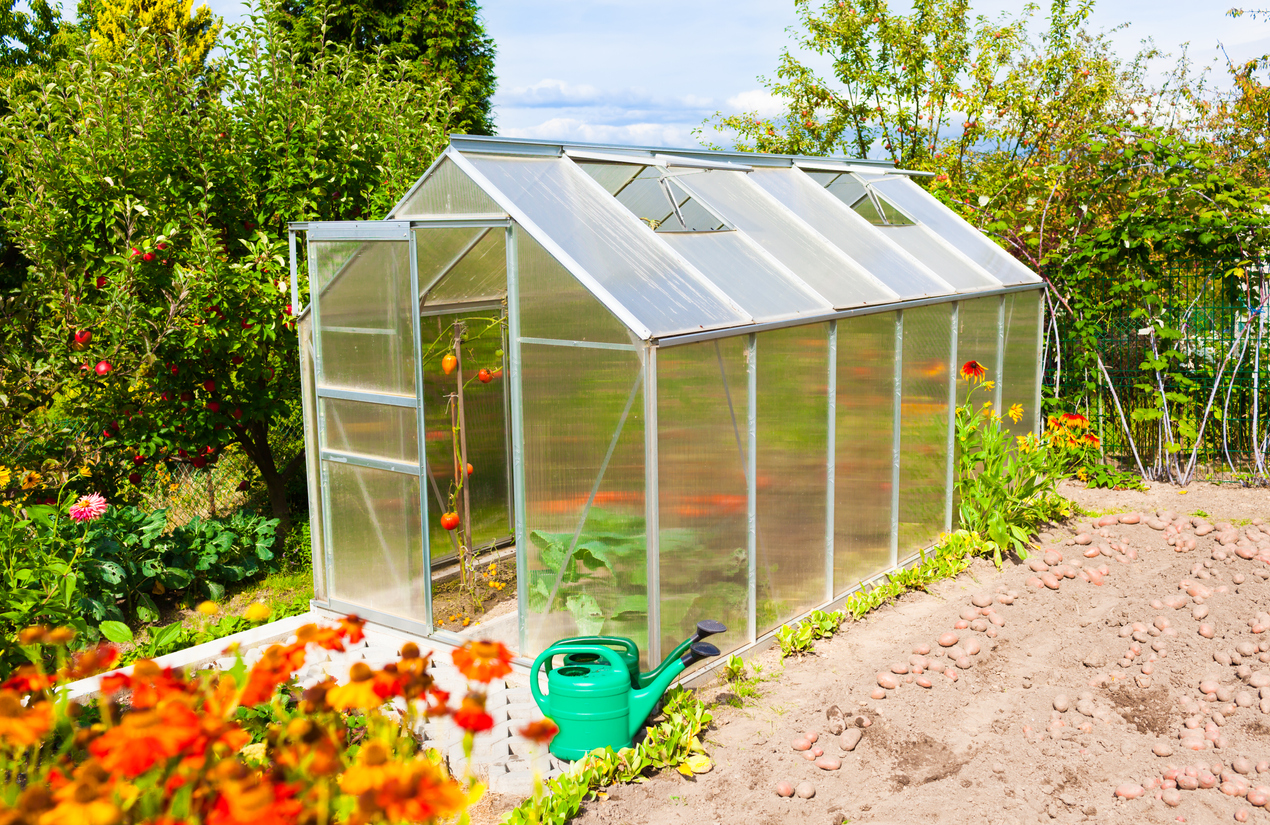
\includegraphics[width=.7\textwidth]{../Figures/invernadero1.jpg}
\caption{Invernadero hogareño}
\label{fig:imgInvernadero}
\end{figure}


%----------------------------------------------------------------------------------------

\section{Estado del arte}
\label{sec:Estado del arte}

Los viveros automatizados o inteligentes se han vuelto sumamente populares entre los aficionados y dueños de pequeños invernaderos debido a su capacidad de mejorar el crecimiento de las plantas minimizando la cantidad de trabajo manual requerido. Una de las características principales de un vivero inteligente es la capacidad de controlar automáticamente factores ambientales como la temperatura, la humedad, la luz y el riego. Esto se puede lograr mediante el uso de sensores, actuadores y controladores que pueden ajustar las condiciones en función de configuraciones preprogramadas o datos en tiempo real. 
En términos de control de temperatura, los viveros inteligentes pueden usar dispositivos como termostatos, ventiladores y calentadores para mantener el rango de temperatura ideal para el crecimiento de las plantas. La humedad se puede regular mediante humidificadores o deshumidificadores, mientras que la iluminación se puede controlar mediante el uso de temporizadores o sensores de luz. También se pueden implementar sistemas de riego controlados. En sistemas mas avanzados, se pueden controlar variables como el suministro de nutrientes, la regulación del dióxido de carbono y los sistemas de control de plagas. 




%\begin{table}[h]
%\centering
%\caption[Análisis del estado del arte]{Análisis del mercado.}
%
%\begin{tabular}{p{0.15\linewidth} | p{0.35\linewidth} | p{0.08\linewidth} | p{0.28\linewidth}}
%\toprule
%\textbf{Proveedor} & 
%\textbf{Características principales} & 
%\textbf{Costo} & 
%\textbf{Tamaño del mercado}\\
%\midrule
%Priva &
%  Sistemas integrales que incluyen gestión de clima, riego y energía.  &
%  \$\$\$\$ &
%  Grande, con una fuerte presencia en Europa y América del Norte. \\
%Hortimax &
%  Sistemas de control para clima, riego y gestión laboral.\ &
%  \$\$\$\$ &
%  Grande, con una fuerte presencia en Europa y Asia. \\
%Argus Controls &
%  Sistemas de automatización para clima, riego y fertirrigación.\ &
%  \$\$ &
%  Grande, con una fuerte presencia  América del Norte. \\ 
%Grodan &
%  Soluciones de riego, fertirrigación y control climático.\ &
%  \$\$ &
%  Grande, con una fuerte presencia en Europa y América del Norte. \\
%Heliospectra &
%  Sistemas de control de iluminación y aplicaciones agrícolas en interiores.\ &
%  \$\$\$\$ &
%  Pequeño, pero en crecimiento con presencia global. \\
%Growlink &
%  Controles inteligentes de temperatura, humedad, CO2, iluminación y riego.\ &
%  \$ &
%  Pequeño, pero en crecimiento con soluciones ajustables a cualquier tamaño. \\ 
%\bottomrule
%\hline
%\end{tabular}
%\label{tab:vendors}
%\end{table}


\begin{table}[h]
\centering
\caption[Análisis del estado del arte]{Análisis del mercado.}

\begin{tabular}{lcccccc} 
\toprule
%\textbf{Funcionalidad} & \textbf{Priva []} & \textbf{Hortimax []} & \textbf{Argus Controls []} &\textbf{Grodan []} & \textbf{Heliospectra []} & \textbf{Growlink []}\\
\textbf{Funcionalidad} & \textbf{Priva []}  & \textbf{Argus Controls []} &\textbf{Grodan []} & \textbf{Growlink []}\\

\midrule
Gestión de clima   & Sí & Sí & Sí & Sí \\
Control de riego   & Sí & Sí & Sí & Sí \\
Fertirrigación     & No & Sí & Sí & ? \\
Gestión de energía & Sí & ? & Sí & Si \\
Tamaño de mercado  & Grande &  Grande & Grande & Pequeño \\
Costo              & \$\$\$\$ &  \$\$ & \$\$ &  \$\$ \\
\bottomrule
\hline
\end{tabular}
\label{tab:vendors}
\end{table}

%----------------------------------------------------------------------------------------

\section{Objetivos y alcance}


El propósito de este trabajo es el desarrollo de un sistema de sensores y actuadores para el control de clima y riego de un vivero. Los mismos deberán comunicarse con una aplicación instalada en un servidor local donde se configurarán los parámetros y alarmas del sistema.

Con el propósito de disponer de un prototipo completo del sistema se incluyó:
 
\begin{itemize}
	\item Sistema para el monitoreo y control de dispositivos IoT.
	\item Sistema de control de usuarios, permisos y accesos a la plataforma.
	\item Interfaz gráfica para acceso y control de la plataforma.
	\item Instrucciones y/o tutoriales para facilitar el uso del sistema.
	\item Análisis, investigación y elección del hardware para los sensores y actuadores.


\end{itemize}


El presente trabajo no incluyó:
\begin{itemize}
	\item Implementación en sitio de los sistemas desarrollados.
	\item Implementación de métodos de control basados en condiciones climatológicas externas.
	\item Desarrollo o implementación de modelos analíticos o predictivos de las condiciones del vivero.
	\item Desarrollo o implementación de conexiones que no sean por Wi-Fi (LTE/5G). 
	
\end{itemize}
\chapter{Introducción específica} % Main chapter title

\label{Chapter2}

%----------------------------------------------------------------------------------------
%	SECTION 1
%----------------------------------------------------------------------------------------
En este capítulo se describen las tecnologías y los protocolos de comunicación, los componentes de hardware, las herramientas de software y los requerimientos para la realización del proyecto.

\section{Tecnologías de comunicación}
\label{sec:Tecnologías de comunicación}
Los principales protocolos de IoT empleados en el trabajo y su posicionamiento en la pila de comunicaciones se muestran resaltados en la figura \ref{fig:IotProtocols}.

%A continuación se describen los principales protocolos empleados en el trabajo. En la figura \ref{fig:IotProtocols} se observa su posicionamiento en la pila de protocolos para IoT.

\begin{figure}[h]
	\centering
	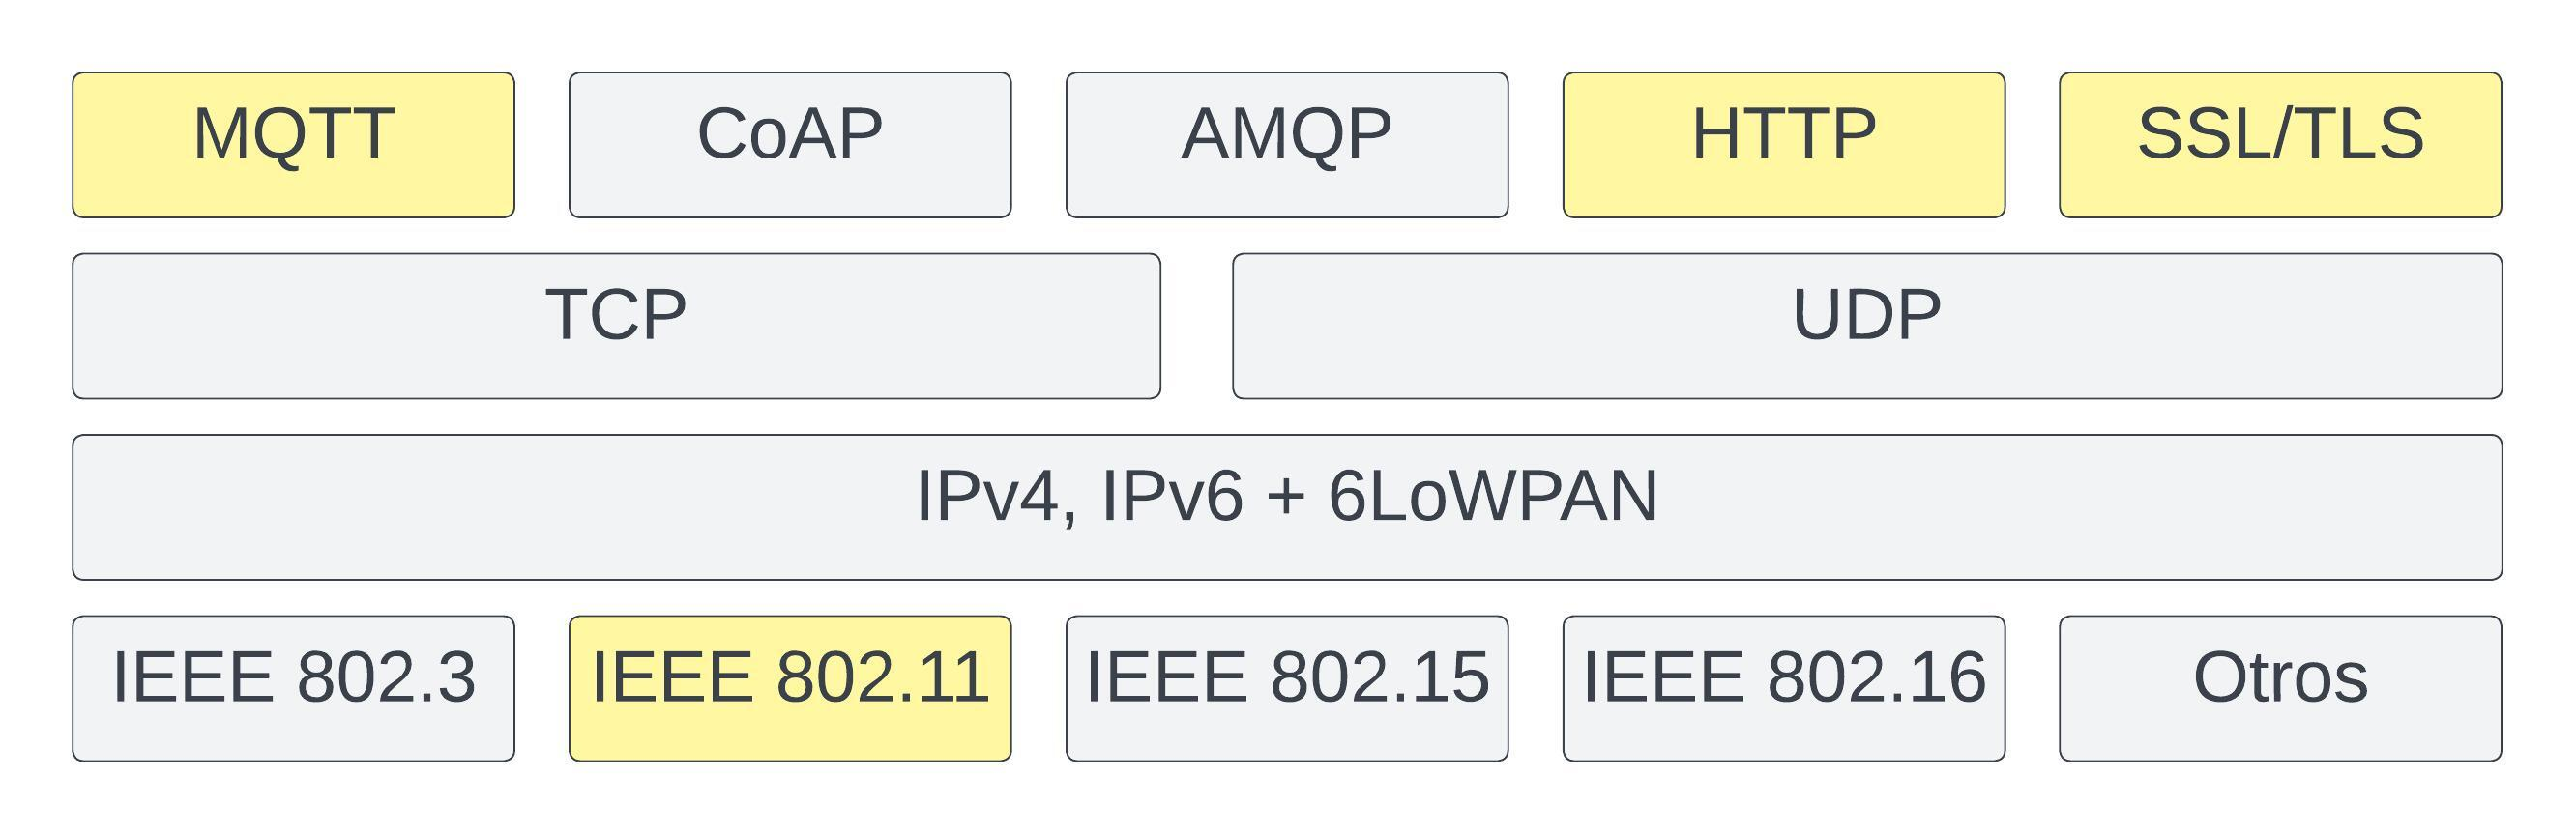
\includegraphics[width=0.75\textwidth]{./Figures/protocols.jpeg}
	\caption[Pila de protocolos para IoT.]{Pila de protocolos para IoT\protect\footnotemark.}
	\label{fig:IotProtocols}

\end{figure}
	\footnotetext{Gráfico creado en base a una imagen tomada de \citep{8088251}}

\subsection{Tecnologías Wi-Fi}
\label{sec:Tecnologías Wi-Fi}
El estándar IEEE 802.11 para redes inalámbricas de área local (WLAN) es conocido comercialmente como Wi-Fi y presenta dos modos de operación \citep{wifi}:
\begin{itemize}
\item Infraestructura: uno o más \textit{access points} (AP) actúan como puente entre la red cableada y la red inalámbrica. Todas las comunicaciones entre los dispositivos conectados a la red se realizan a través de los APs. 
\item Ad-hoc: cada nodo puede realizar una conexión directa con otro, sin necesidad de un AP central. En este caso, los nodos se organizan en una red donde todos son capaces de enrutar los paquetes.  
\end{itemize}

\subsection{Protocolo MQTT}
\label{sec:Protocolo MQTT}

MQTT fue desarrollado en 1999 con el objetivo principal de crear un protocolo muy eficiente desde el punto de vista del uso del ancho de banda y de muy bajo consumo de energía. Por estas razones es adecuado para el uso en IoT \citep{mqtt:1}.

Su funcionamiento se basa en el paradigma de publicación-suscripción que consiste en desvincular un cliente que publica un mensaje (publicador) de otros clientes que reciben el mensaje (suscriptores). Sumado a esto, MQTT es un protocolo asincrónico, lo que significa que el cliente puede seguir operando mientras espera un nuevo mensaje.

Un componente principal del protocolo es el \textit{broker} cuya función primaria es la de recibir los mensajes de los publicadores y enviarlos a los  suscriptores. Para realizar esta tarea, el \textit{broker} utiliza temas o \textit{topics} para agrupar clientes que necesitan recibir los mismos mensajes. De esta manera, el \textit{topic} es un canal virtual que conecta a los publicadores con sus suscriptores \citep{mqtt:1}.

En la figura \ref{fig:arqmqtt} se observa la arquitectura del protocolo.
\begin{figure}[h]
	\centering
	\includegraphics[width=0.75\textwidth]{./Figures/mqtt.jpeg}
	\caption[Arquitectura del protocolo MQTT.]{Arquitectura del protocolo MQTT\protect\footnotemark.}
	\label{fig:arqmqtt}

\end{figure}

	\footnotetext{Gráfico creado en base a una imagen tomada de  \citep{mqtt:1}}


\subsection{Protocolo HTTP}
\label{sec:Protocolo HTTP}

El \textit{Hypertext Transfer Protocol} (HTTP)\citep{http:1} es un protocolo utilizado en la Web para el desarrollo de aplicaciones y está basado en el paradigma cliente-servidor. Aquí el cliente emplea un agente intermediario (por lo general un \textit{browser}) para realizar un pedido de información y el servidor proporciona una respuesta. Esto se conoce con el nombre de modelo \textit{request/response}.

HTTP es un protocolo que no guarda información de estado, esto significa que el servidor no es capaz de reconocer la relación entre múltiples pedidos de un mismo usuario  \citep{oreilly:1}.

En la actualidad, HTTP se utiliza en conjunto con la arquitectura REST (\textit{Representational State Transfer}) \citep{rest} para facilitar la interacción entre distintas entidades sobre servicios basados en red. Esta asociación permite que los dispositivos interactúen mediante funciones estándares de tipo CRUD (\textit{create, read, update, delete})  \citep{10.1145/3292674}. Dichas funciones a su vez se traducen a los métodos HTTP POST, GET, PUT y DELETE respectivamente \citep{GLAROUDIS2020107037}. 

\subsection{Protocolo SSL/TLS}
\label{sec:Protocolo SSL/TLS}
\textit{Secure Socket Layer/Transport Layer Security} (SSL/TLS) \citep{tls:1} es un protocolo criptográfico que proporciona seguridad de extremo a extremo de los datos enviados entre aplicaciones a través de Internet.
TLS evolucionó a partir de \textit{Secure Socket Layer} (SSL), que fue desarrollado originalmente por Netscape Communications Corporation en 1994 para proteger las sesiones web. 

SSL 1.0 nunca se lanzó públicamente, mientras que SSL 2.0 fue reemplazado rápidamente por SSL 3.0 que proporcionó las bases para la posterior creación de TLS. 

Cabe señalar que TLS no protege los datos en los sistemas finales, simplemente garantiza la entrega segura de datos a través de Internet y al mismo tiempo evita posibles escuchas y/o alteraciones del contenido.
TLS normalmente se implementa sobre TCP \citep{rfc793} para cifrar los protocolos de la capa de aplicación, como por ejemplo HTTP.

TLS utiliza una combinación de criptografía simétrica y asimétrica que proporciona un buen compromiso entre rendimiento y seguridad al momento de transmitir la información \citep{tls:2}. Para mayor protección es deseable que un cliente que se conecta a un servidor pueda validar la veracidad de la clave pública ofrecida por este. Normalmente dicha verificación se lleva a cabo por medio de un certificado digital X.509 \citep{x509:1} emitido por un tercero de confianza denominado Autoridad Certificadora (CA). Dicha CA está encargada de  afirmar la autenticidad de la clave pública. En los casos en los que no se dispone de una CA, un servidor puede usar un certificado autofirmado en el que el cliente debe confiar explícitamente \citep{tls:2}.


En la figura \ref{fig:ssl2way} se detalla el esquema de autenticación y verificación con certificados e inicio de una conexión segura.

\begin{figure}[h]
	\centering
	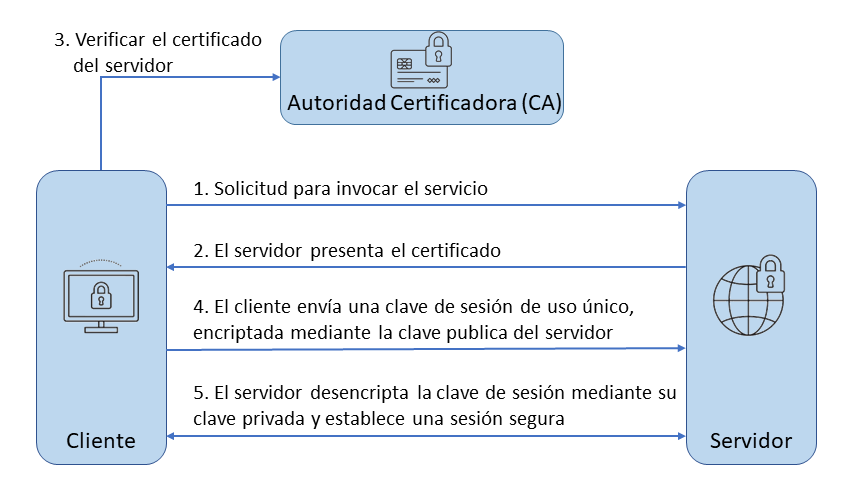
\includegraphics[width=0.9\textwidth]{./Figures/tls.png}
	\caption[Proceso de autenticación de TLS]{Proceso de autenticación de TLS\protect\footnotemark.}
	\label{fig:ssl2way}

\end{figure}
	\footnotetext{Gráfico creado en base a una imagen tomada de http://www.herongyang.com/PKI/HTTPS-Communication-Data-Encryption.html}
	
\section{Componentes de hardware utilizado}
\label{sec:Hardware utilizado}

\subsection{Raspberry Pi}
\label{sec:Raspberry Pi}
Se denomina así a una serie de computadoras monoplaca o computadoras de placa simple (SBC, por \textit{Single Board Computer}) de bajo costo desarrollados por la Raspberry Pi Foundation \citep{raspberrypi:1}.
Una de sus principales características es proveer un conjunto de pines de GPIO (\textit{general purpose input/output} que permiten controlar componentes electrónicos y otros dispositivos en el ámbito de Internet de las Cosas.
A pesar de su reducido tamaño, la Raspberry Pi ofrece una capacidad de procesamiento comparable a una computadora de escritorio y es por ello que su uso se ha expandido en proyectos que incluyen domótica, \textit{edge computing} o aplicaciones industriales \citep{raspberrypi:2}. 

En la figura \ref{fig:rpi} se muestra una Raspberry Pi modelo 4B similar a la utilizada en el trabajo y en la tabla \ref{tab:raspberrypi} se listan sus principales características: 
 
\begin{table}[h]
\centering
\caption[Especificaciones técnicas de la Raspberry Pi 4B.]{Especificaciones técnicas de la Raspberry Pi 4B.}

\begin{tabular}{p{3cm} p{8cm}} 
\toprule
\textbf{Categoría} & \textbf{Especificación}\\

\midrule
Procesador	& Broadcom BCM2711, quad-core Cortex-A72 (ARM v8) 64 bits SoC @ 1,8 GHz \\
Memoria SDRAM	 & 1, 2, 4 u 8 GB LPDDR4-3200 \\
Wi-Fi	& 2,4 GHz and 5,0 GHz IEEE 802.11ac \\
Bluetooth	&  5.0, BLE \\
Ethernet	& Gigabit, con soporte opcional para POE\\
USB	& 2 puertos  3.0 ; 2 puertos 2.0\\
GPIO	&	Conector de 40 pines\\
HDMI	&  2 puertos micro-HDMI\\
Alimentación	& 5 V USB y GPIO\\
Temperatura	& 0 °C a 50 °C \\
\bottomrule
\hline
\end{tabular}
\label{tab:raspberrypi}
\end{table}
 
\begin{figure}[h]
	\centering
	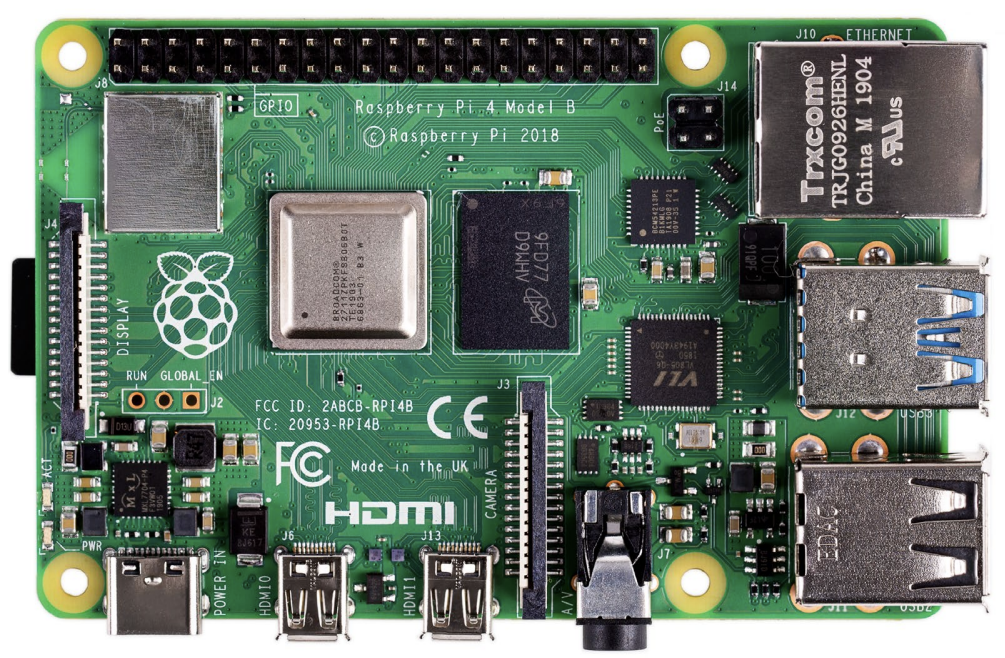
\includegraphics[width=0.75\textwidth]{./Figures/rpi.png}
	\caption[Raspberry Pi.]{Raspberry Pi\protect\footnotemark.}
	\label{fig:rpi}
\footnotetext{Imagen tomada de https://datasheets.raspberrypi.com/.}
\end{figure}

\subsection{Módulos ESP}
\label{sec:Módulos ESP}
ESP es una familia de microcontroladores de baja potencia  desarrollada por la empresa china Espressif. Estos chips cuentan con una amplia variedad de usos en IoT tanto en el ámbito profesional/industrial como en el de los aficionados \citep{esp32} \citep{esp8266}. 

En la tabla \ref{tab:esp} se observa una comparación entre los modelos ESP32-WROOM-32 y ESP8266 utilizados en este trabajo.





\begin{table}[h]
\centering
\caption[Especificaciones de los microcontroladores ESP.]{Especificaciones de los microcontroladores ESP.}

\begin{tabular} {p{4.5cm} p{3.7cm} p{3.7cm}} 
\toprule
\textbf{Características} & \textbf{ESP32} \citep{esp32}  & \textbf{ESP8266} \citep{esp8266} \\
\midrule
Procesador		& 2 x Xtensa 32 bits LX6	& Tensilica L106 32 bits\\
Memoria ROM	 	& 448 KB	& No dispone\\	
Memoria SRAM	& 520 KB	& 160 KB\\
Wi-Fi			& 802.11 b/g/n & 802.11 b/g/n\\
Bluetooth		& 4.2, BLE & No dispone\\
GPIOs			& 34 pines & 17 pines\\
Consumo normal	& \textasciitilde 500 mA & \textasciitilde 80 mA \\
Temperatura de operación		& -40 °C a 85 °C & -40 °C a 125 °C \\
Sistema operativo &	freeRTOS	& freeRTOS \\
Costo en USD	& \$ 6 a \$ 12  & \$ 3 a  \$ 6 \\
\bottomrule
\hline
\end{tabular}
\label{tab:esp}
\end{table}

El modelo ESP8266 es una versión anterior al ESP32 y ofrece una menor variedad de características que este último. Sin embargo, constituye una opción económica cuando los requerimientos de conectividad y rendimiento van de la mano con sus prestaciones.

 

En la figura \ref{fig:esp32} se observa un módulo de desarrollo de la familia ESP32.



\begin{figure}[h]
	\centering
	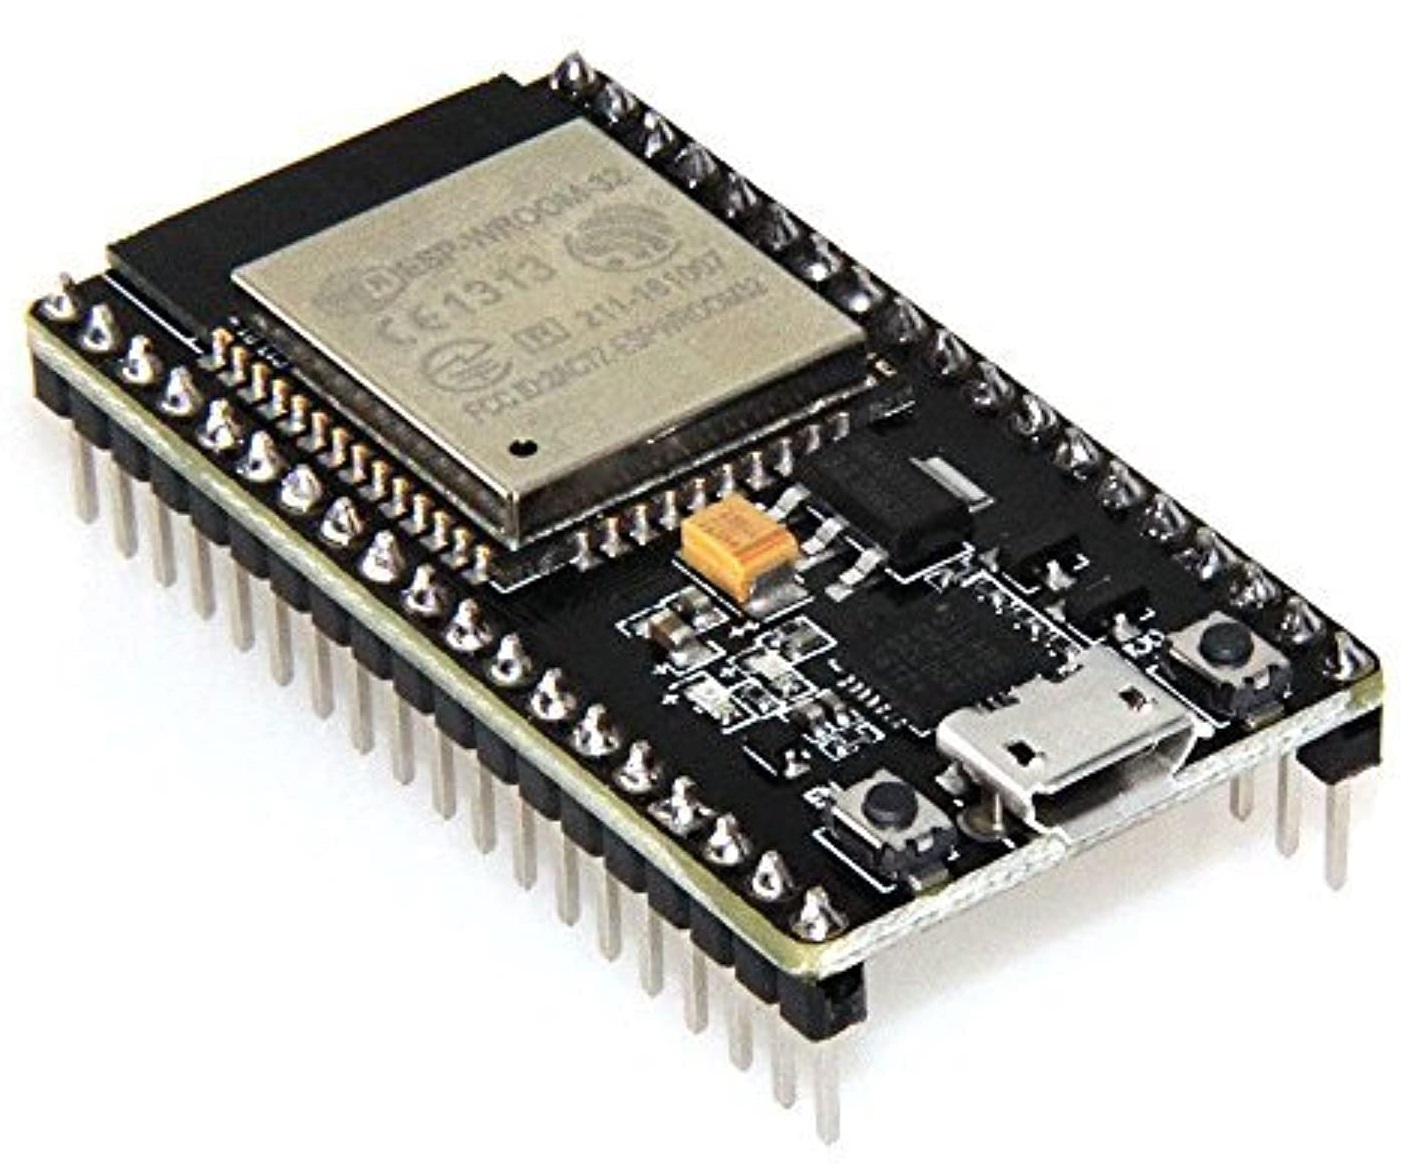
\includegraphics[width=0.30\textwidth]{./Figures/esp32.jpg}
	\caption[Módulo de desarrollo ESP32.]{Módulo de desarrollo ESP32.}
	\label{fig:esp32}

\end{figure}

\subsection{Sensores y actuadores}
\label{sec:Sensores y actuadores}
Los principales sensores y actuadores empleados en el sistema del invernadero inteligente son los siguientes:
\begin{itemize}

\item DHT22: módulo básico y económico para determinar los valores de temperatura y humedad en forma digital. Utiliza un sensor de humedad capacitivo y un termistor para medir el aire circundante y entrega una señal digital en el pin de datos de acuerdo al valor calculado. Funciona con una alimentación de 3,3 a 6 VDC y su rango de medición es de -40 °C a 80 °C y de 0 a 100 \% de humedad relativa \citep{dht22}.

\item Sensor capacitivo de humedad del suelo: compuesto de un material resistente a la corrosión, mide la humedad del suelo indirectamente por medio de la capacidad observada. Opera con una alimentación de 3,3 a 5,5 VDC \citep{soilsensor}.

\item Válvula solenoide de dos vías: dispositivo neumático para controlar el flujo de líquidos o gases que se acciona eléctricamente. Para poder operarlo, se utiliza un relé que es un instrumento electromecánico que actúa como interruptor controlado por un circuito eléctrico \citep{valve}\citep{rele}.

La figura \ref{fig:sensores} muestra imágenes de los componentes listados previamente.

\end{itemize}
%\begin{figure}[h]
%	\centering
%	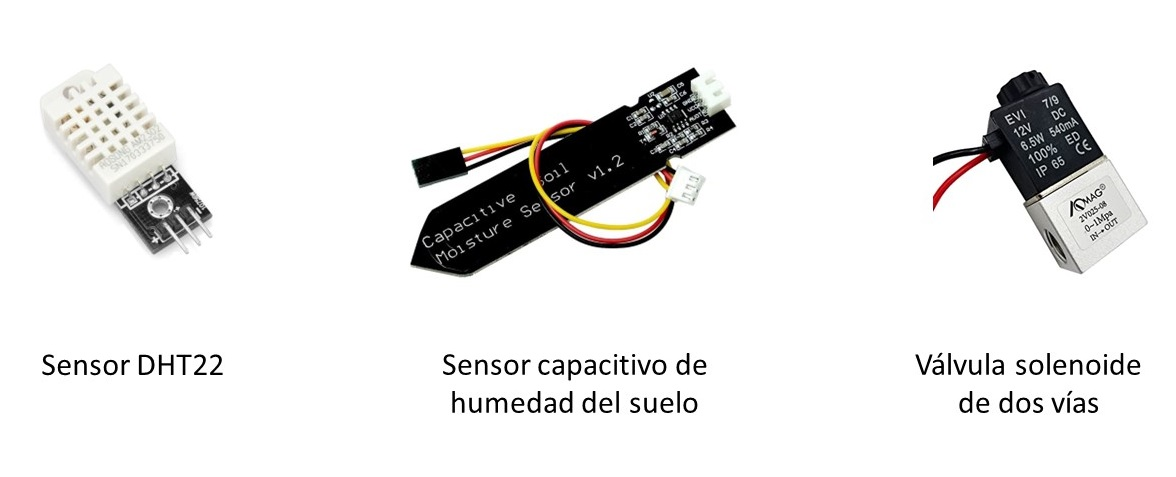
\includegraphics[width=0.90\textwidth]{./Figures/sensores.jpg}
%	\caption[Principales sensores y actuadores empleados en el invernadero.]{Principales sensores y actuadores empleados en el invernadero.}
%	\label{fig:sensores}
%
%\end{figure}

\begin{figure}[!htpb]
     \centering
     \begin{subfigure}[b]{0.3\textwidth}
         \centering
         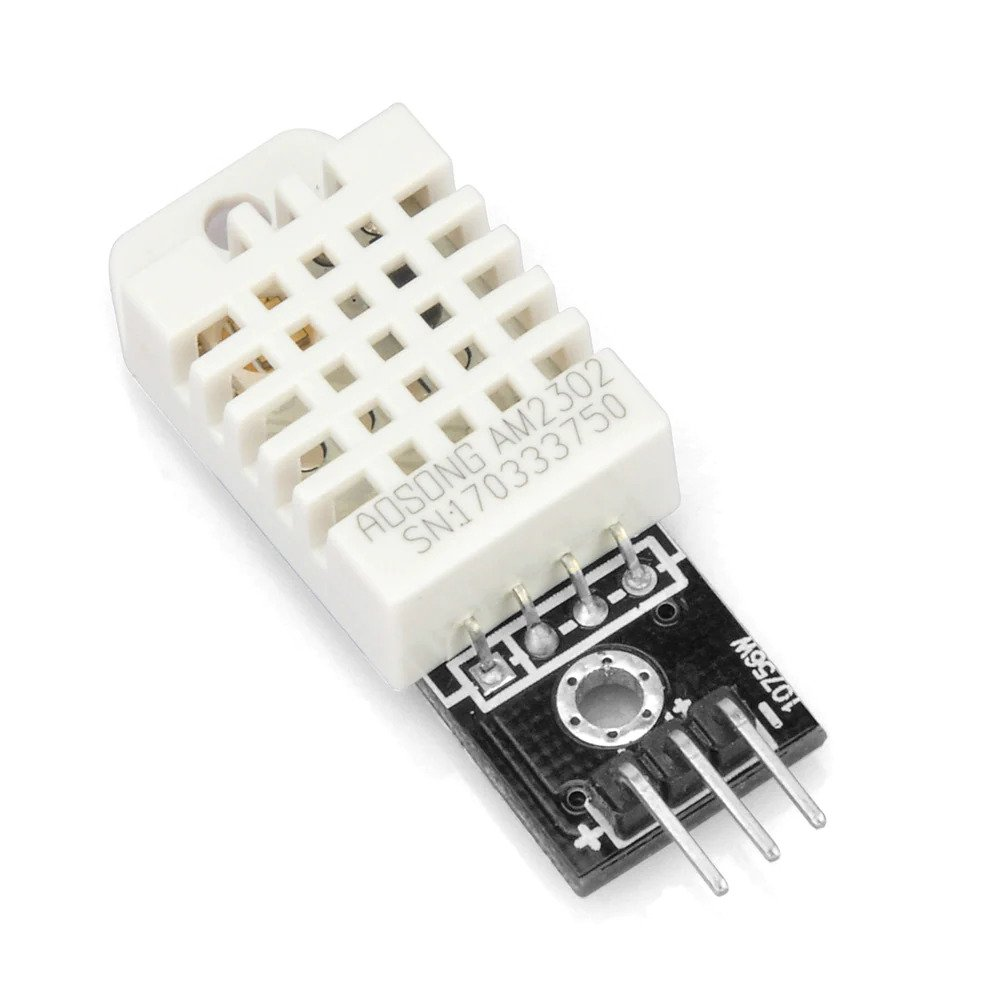
\includegraphics[width=.65\textwidth]{./Figures/dht22.jpg}
         \caption{Sensor de temperatura y humedad.}
         \label{fig:dht22}
     \end{subfigure}
     \hfill
     \begin{subfigure}[b]{0.3\textwidth}
         \centering
         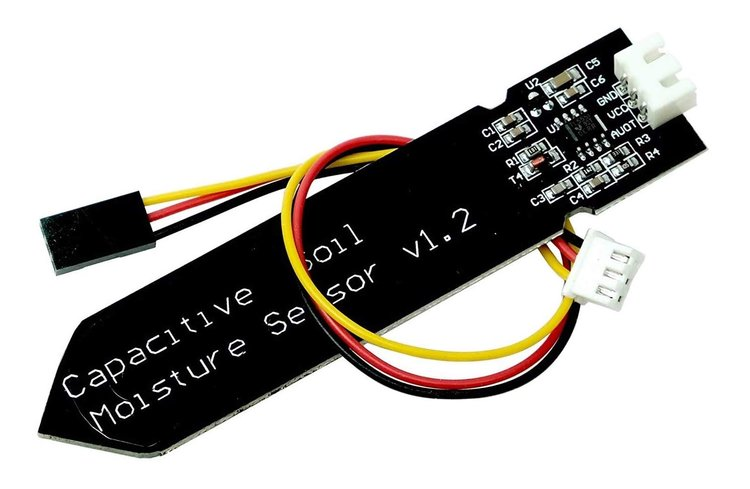
\includegraphics[width=.65\textwidth]{./Figures/soilsensor}
         \caption{Sensor de humedad del suelo.}
         \label{fig:soilsensor}
     \end{subfigure}
     \hfill
     \begin{subfigure}[b]{0.3\textwidth}
         \centering
         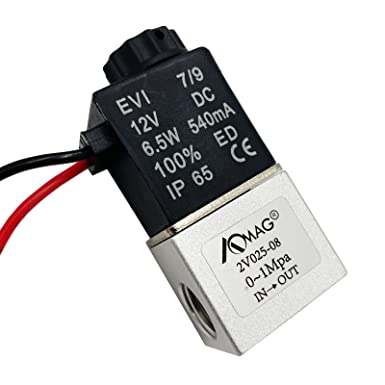
\includegraphics[width=.65\textwidth]{./Figures/valve.jpg}
         \caption{Válvula solenoide de dos vías.}
         \label{fig:valve}
     \end{subfigure}
        \caption[Principales sensores y actuadores empleados en el invernadero.]{Principales sensores y actuadores empleados en el invernadero.}
        \label{fig:sensores}
\end{figure}




\section{Tecnologías de software aplicadas}
\label{sec:Software aplicado}
\subsection{ThingsBoard}
\label{sec:ThingsBoard}
ThingsBoard es una plataforma de código abierto que permite el desarrollo, administración y expansión de proyectos de IoT. Esta aplicación permite la gestión de las comunicaciones, el almacenamiento y la visualización de los datos que provienen de los sensores u otros dispositivos que formen parte del sistema \citep{thingsboard:1}.
Se ofrece en las siguientes versiones:
\begin{itemize}

\item Professional Edition: es la versión comercial, con varios tipos de licenciamiento y costos según sea el sistema a implementar. Esta edición posee soporte técnico, ilimitada cantidad de dispositivos a conectar y soporte para almacenamiento híbrido entre otras funcionalidades.

\item Cloud: similar a la edición profesional, pero alojada en la nube de ThingsBoard. En este caso el proveedor se encarga del manejo de los componentes de la plataforma.
 
\item Community edition: es la edición libre de licenciamientos y la que se utilizó en este trabajo. Si bien no tiene limitaciones en cuanto a la cantidad de dispositivos a conectar, carece de ciertas funcionalidades como por ejemplo la descarga de datos de dispositivos desde la interfaz web o la ejecución programada de tareas (\textit{scheduler}).
\end{itemize}
%
%\begin{table}[h]
%\centering
%\caption[Comparación de versiones de ThingsBoard]{Especificaciones técnicas de Raspberry PI 4B}
%
%\begin{tabular}{p{0.30\textwidth} p{0.15\textwidth} p{0.15\textwidth} p{0.15\textwidth}} 
%\toprule
%\textbf{Categoría} & \textbf{Community Edition} & \textbf{Professional Edition} & \textbf{Cloud}\\
%
%\midrule
%Gestión de activos y recopilación de datos				&	Sí &	Sí &	Sí\\
%Paneles de control en tiempo real para usuarios finales &	Sí &	Sí &	Sí\\
%Cadenas de reglas personalizables, widgets				&	Sí &	Sí &	Sí\\
%Transporte MQTT, HTTP, CoAP, OPC-UA						&	Sí &	Sí &	Sí\\
%Integraciones con sistemas BigData						&	Sí &	Sí &	Sí\\
%Soporte NB-IoT, SigFox, LoRaWAN				&	Sí &	Sí &	Sí\\
%Motor de reglas							& Básico & Avanzado & Avanzado\\
%Grupos de entidades										& Básico & Avanzado & Avanzado	\\	
%RBAC avanzado para IoT									&	No & Sí & Sí\\
%\textit{Scheduler}										&	No & Sí & Sí	\\
%Reportes												&	No & Sí & Sí\\
%Personalización de marca								&	No & Sí & Sí\\
%Exportación de datos							&	No & Sí & Sí\\
%Integraciones								&	No & Sí & Sí\\
%Gestión de dominios										&	No	& No & No\\
%\bottomrule
%\hline
%\end{tabular}
%\label{tab:raspberrypi}
%\end{table}

\subsection{Arduino IDE}
\label{sec:Arduino IDE}

Arduino IDE (\textit{Integrated Development Environment}) es un software de código abierto que se utiliza para escribir y cargar código a placas Arduino. Sin embargo por medio de la instalación de paquetes de expansión, el IDE soporta hardware de terceros entre los que encuentran las módulos ESP32/ESP8266 \citep{Arduinosupport} empleados en este proyecto.

El código de los programas se realiza en lenguaje C o C++ y los archivos resultantes se denominan \textit{sketches}. Estos son compilados y cargados en las placas desde el mismo IDE \citep{arduinoide}.

Este software es una herramienta fácil de utilizar tanto por usuarios experimentados como por principiantes. Es frecuentemente empleada por aquellos que se inician en la programación electrónica y la robótica o al momento de construir prototipos interactivos \citep{arduinoide:2}. 

\subsection{Telegram}
\label{sec:Telegram}

Telegram es una aplicación de mensajería multiplataforma rápida, simple y gratuita. Está basada en la nube y cuenta con sincronización constante, lo que significa que se puede acceder a los mensajes desde diferentes dispositivos simultáneamente. 

Tanto el código de los clientes de Telegram como el de su API son abiertos, lo que permite crear otras aplicaciones a partir de ellos. Adicionalmente cuenta con una API para \textit{bots} que facilita la implementación de herramientas basadas en Telegram, la integración de servicios o la realización pagos \citep{telegram}.
 
  

\section{Requerimientos}
\label{sec:Requerimientos}

A continuación se listan los principales requerimientos funcionales,  no funcionales y de documentación del proyecto:

\begin{itemize}
\item Requerimientos funcionales:
\begin{enumerate}

\item El estado del sistema podrá ser consultado desde Internet.
\item La aplicación soportará múltiples usuarios de forma concurrente.
\item La aplicación permitirá crear roles de usuarios con diferentes permisos.
\end{enumerate}
\end{itemize} 
\begin{itemize}
\item Requerimientos no funcionales:
\begin{enumerate}
\item El rango de tensión de alimentación de los nodos será de 3,3 a 5 VDC.
\item El sistema de riego operará con una tensión de alimentación de 12 VDC.
\item El sistema estará basado en software de código abierto.
\item El firmware deberá desarrollarse en plataformas de código abierto.
\item El trabajo se realizará sobre dispositivos de bajo costo y fácil reposición.
\item Los datos se almacenarán localmente.
\item La aplicación soportará MQTT.
\item Los sensores de humedad del suelo tendrán una protección IP65 \citep{ip65}. 
\end{enumerate}


\end{itemize} 
\begin{itemize}
\item Requerimientos de documentación:
\begin{enumerate}
\item Los manuales y/o guías estarán redactados en inglés.
\end{enumerate}


\end{itemize}
 


\chapter{Diseño e implementación} % Main chapter title

\label{Chapter3} % Change X to a consecutive number; for referencing this chapter elsewhere, use \ref{ChapterX}



En este capítulo se presentan los detalles del diseño de los nodos sensores y actuadores que conforman el trabajo, como así también los del software seleccionado.

\section{Arquitectura de la solución}
\label{sec:Arquitectura de la solución}

%Como se observa en la figura \ref{fig:blockdiagram}, el invernadero inteligente está compuesto por un conjunto de subsistemas encargados de las diferentes funciones de medición y control de variables, una aplicación central y un sistema que permita el acceso remoto de forma segura.

Para la implementación del prototipo propuesto en el trabajo se requirió la construcción de diferentes subsistemas encargados de las múltiples funciones dentro del invernadero inteligente. Cada uno de ellos opera en forma independiente del resto y se comunican con una aplicación central mediante una red inalámbrica. 
Para garantizar el acceso de los usuarios desde Internet se desarrolló una interfaz de acceso remoto.





\subsection{Componentes del sistema}
\label{Componentes del sistema}

En la figura \ref{fig:blockdiagram} se observa el diagrama en bloques de la arquitectura diseñada, que está compuesta por los siguientes elementos: 

\begin{itemize}
\item Sistema de monitoreo y control de clima, formado por dos módulos:
\begin{itemize}
\item Sensores de temperatura y humedad con sus correspondientes microcontroladores.
\item Unidad de control de temperatura y humedad comprendida por un microcontrolador, relé y ventiladores. 
\end{itemize}
Los sensores miden la temperatura y humedad ambiente en el invernadero y envían estos valores a la aplicación central por medio del microcontrolador. De acuerdo con los datos recibidos, la aplicación determina si es necesario emitir una señal para que la unidad de control encienda los ventiladores.



\item Sistema de control de riego, dividido en dos partes:
\begin{itemize}
\item Conjunto de sensores de humedad de suelo con sus respectivos microcontroladores.
\item Unidad de control de riego constituida por un microcontrolador, relés, bomba de agua y válvulas.
\end{itemize}

Los sensores envían las mediciones a la aplicación central que se encarga de procesarlas. En caso de ser necesario, se disparan las señales de encendido a través de la unidad de control. Primero se activa la válvula que corresponda y luego se enciende la bomba de agua para comenzar el riego. El orden de estas actividades es importante para evitar daños en la bomba o las cañerías.

\item Aplicación central. Constituye el cerebro del invernadero y es la encargada de almacenar los parámetros de configuración de los diversos sensores y actuadores, procesar los mensajes recibidos, disparar acciones y alertas y visualizar el estado general.

\item Sistema de acceso remoto. Permite a los usuarios obtener reportes del sistema en forma segura desde Internet.   
\end{itemize}



\begin{figure}[h]
	\centering
	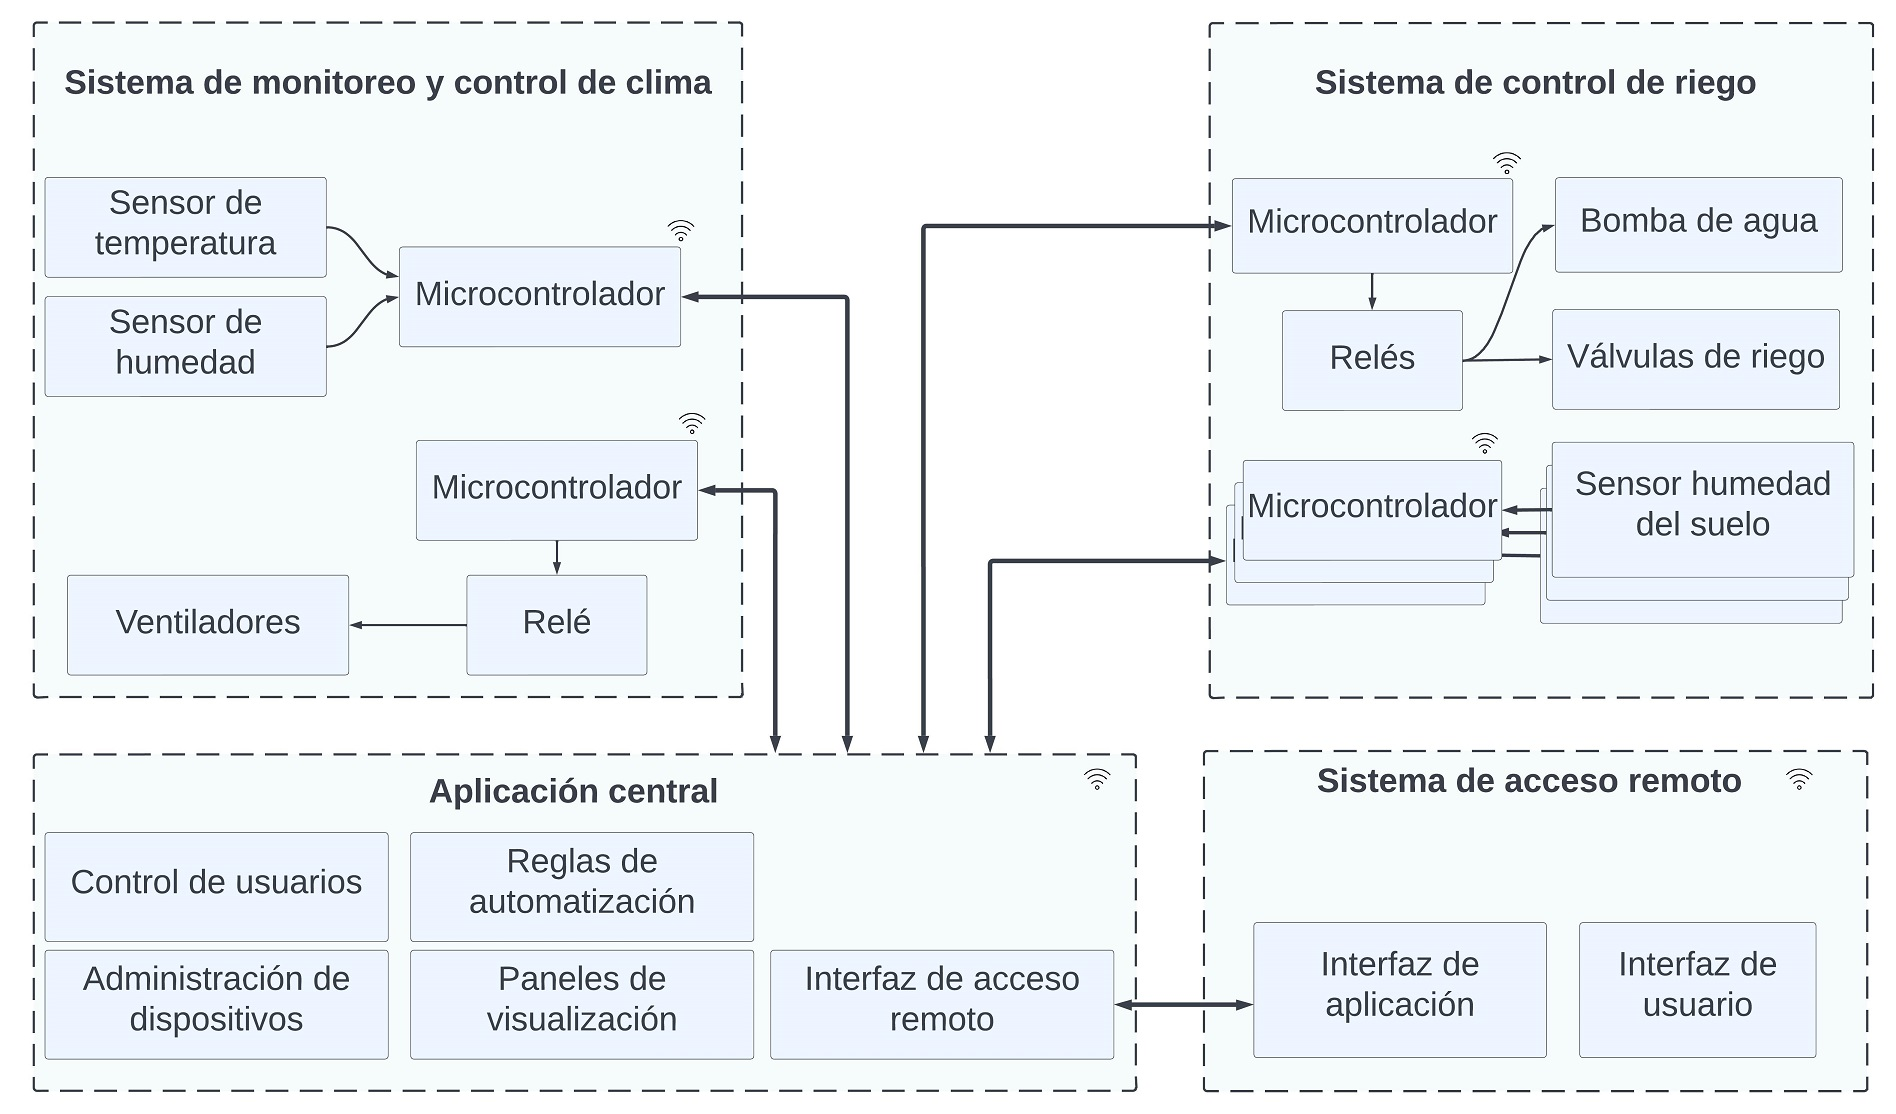
\includegraphics[width=1.0\textwidth]{./Figures/blockdiagram4.jpg}
	\caption[Arquitectura del sistema.]{Arquitectura del sistema.}
	\label{fig:blockdiagram}

\end{figure}


\subsection{Protocolos de comunicación}
\label{Protocolos de comunicación}
%\textit{Aquí se describe cómo se comunican los sistemas con la aplicación central y los protocolos usados en cada caso.}

%En la selección del software de la aplicación central se contempló la compatibilidad con múltiples protocolos de comunicación. Sin embargo limitaciones de configuración específicas, tal como el tiempo de retención de los mensajes en las colas de MQTT, forzaron el utilizar diferentes protocolos dependiendo del módulo en cuestión. Otro factor condicionante, como se detalla en la sección \ref{sec:Ciberseguridad del sistema}, fue el carecer de una CA que emita certificados que todos los componentes puedan confiar.

En esta sección se describe cómo se comunican los sistemas con la aplicación central y los protocolos usados en cada caso. En la figura \ref{fig:blockprotos} se aprecia un esquema simplificado que ilustra dichas interacciones.

Si bien los módulos de hardware y el software soportan una gran variedad de protocolos,  se implementó MQTT en la mayoría de los casos conforme a los requerimientos. En algunas situaciones donde esto no fue técnicamente posible, se utilizó HTTP. Adicionalmente, para garantizar la seguridad de las comunicaciones, se incorporó un certificado autofirmado TLS en el servidor.

\begin{figure}[h]
	\centering
	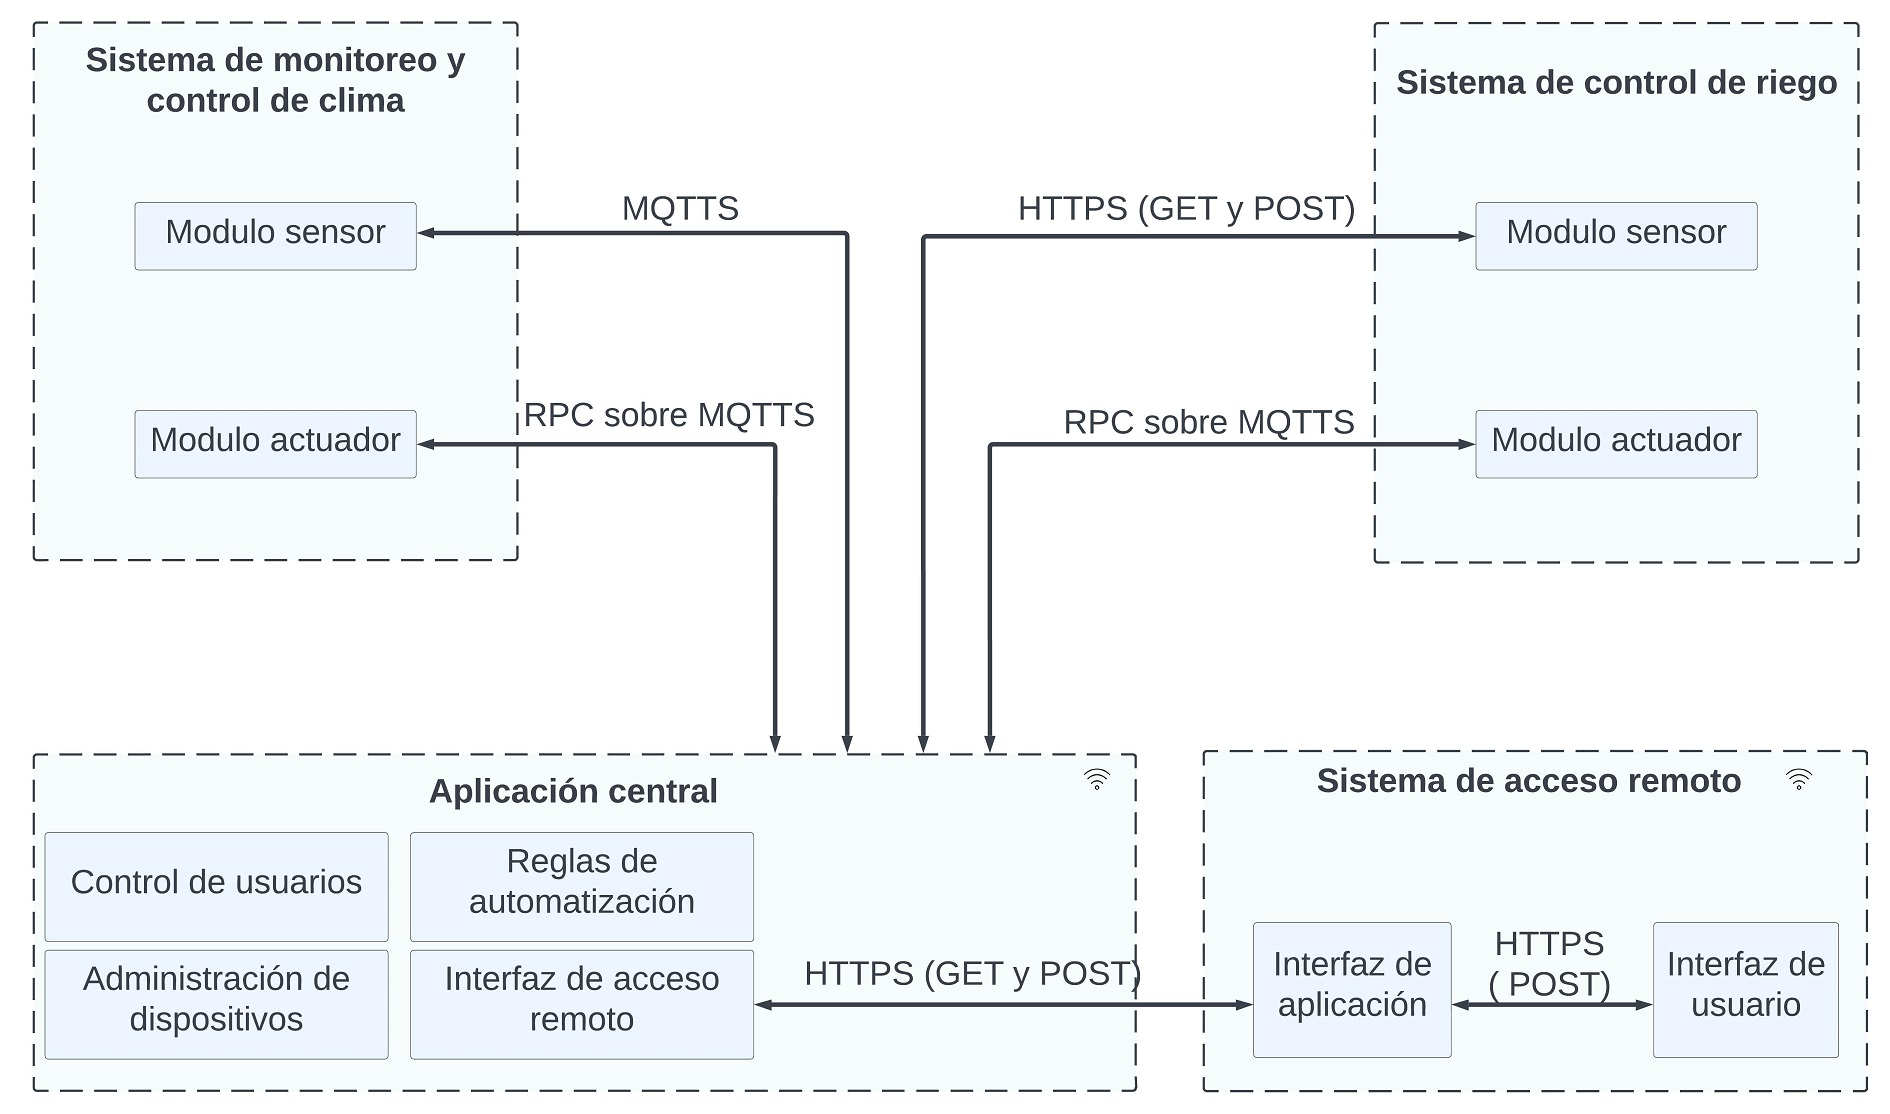
\includegraphics[width=1.0\textwidth]{./Figures/blockproto2.jpg}
	\caption[Protocolos de comunicación entre módulos.]{Protocolos de comunicación entre módulos.}
	\label{fig:blockprotos}
\end{figure}


\pagebreak
Las interacciones principales entre los bloques componentes son:
 
 \begin{itemize}
	\item Sistema de monitoreo y control de clima: las comunicaciones se realizan exclusivamente con aplicación central.
	El módulo sensor envía las mediciones realizadas por medio de MQTT y en caso de requerir una acción, la aplicación central comanda el encendido de los ventiladores por medio de un mensaje enviado por RPC \citep{rfc1057} sobre MQTT.
	
	\item Sistema de control de riego: las comunicaciones se realizan con la aplicación central de manera bidireccional.
	El módulo sensor efectúa dos conexiones, una para el envío de las mediciones y otra para recibir valores de atributos tales como la duración del tiempo de riego. Debido a limitaciones en la configuración de la persistencia de los mensajes en las colas de MQTT, se optó por utilizar llamadas HTTP (GET y POST) para realizarlas.
	Al igual que en el control de clima, la aplicación central inicia el riego por medio de mensajes RCP sobre MQTT hacia el controlador de la bomba y de las válvulas.
	
	\item Sistema de acceso remoto: la interfaz se comunica con la aplicación por medio de pedidos HTTP GET y POST para consultar el reporte de estado de los diferentes componentes. A continuación este se envía hacia la interfaz de usuario por medio de una solicitud HTTP POST.
 
 
 
 
 \end{itemize}






\section{Detalle de los módulos de hardware}
\label{sec:Módulos de hardware}
En esta sección se describen en detalle los esquemas de conexión de los distintos módulos y las consideraciones de diseño y construcción empleadas. 

\subsection{Módulos sensores de humedad del suelo}
\label{Módulos sensores de humedad del suelo}


En el proyecto se desarrollaron dos configuraciones diferentes de módulos para medir la humedad del suelo en macetas de diverso tipo y tamaño. Ambas opciones utilizan el microcontrolador ESP8266 pero incorporan distinta cantidad de sensores. En la figura \ref{fig:soilschem1} se muestra el esquema de conexión para la versión simple (con un único sensor) y en la figura \ref{fig:soilschem2} se ilustra la configuración doble.

Si bien en el prototipo los sensores se conectaron a una fuente de alimentación, la configuración y conexión del sistema está optimizada para el uso de baterías. Esto se debe a que las sondas pueden estar desplegadas en múltiples ubicaciones dentro del invernadero y no siempre es posible conectarlas a la red eléctrica. 

El ahorro de energía necesario para permitir el uso de  baterías se logra a través de ciclos de apagado en los períodos donde no se realizan lecturas. A este mecanismo se lo que conoce como \textit{deep sleep} y una vez que el microcontrolador se encuentra en este estado se requiere un pulso eléctrico en el pin de \textit{reset} para que retorne al modo activo. 
Para habilitar la reactivación se interconectaron los pines D0 (GPIO16) y RST del chip ESP8266. Se logra así una reducción del consumo de energía a valores muy pequeños que rondan los 0,3 mA durante el período de inactividad.




\begin{figure}[!h]
     \centering
     \begin{subfigure}[b]{0.45\textwidth}
		\centering
		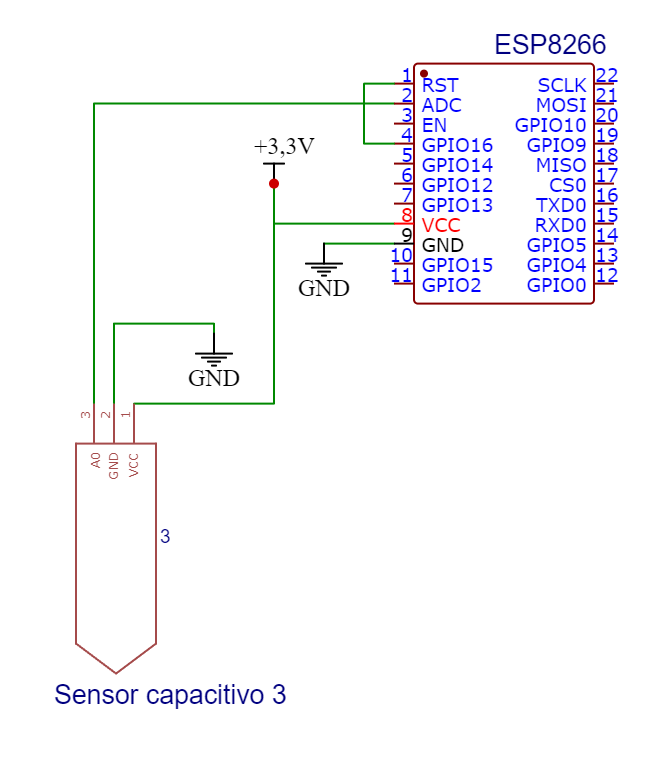
\includegraphics[width=0.9\textwidth]{./Figures/soil_schem_simple.png}
		\caption[Módulo sensor simple]{Módulo sensor simple.}
		\label{fig:soilschem1}
     \end{subfigure}
     \hfill
     \begin{subfigure}[b]{0.45\textwidth}
	\centering
		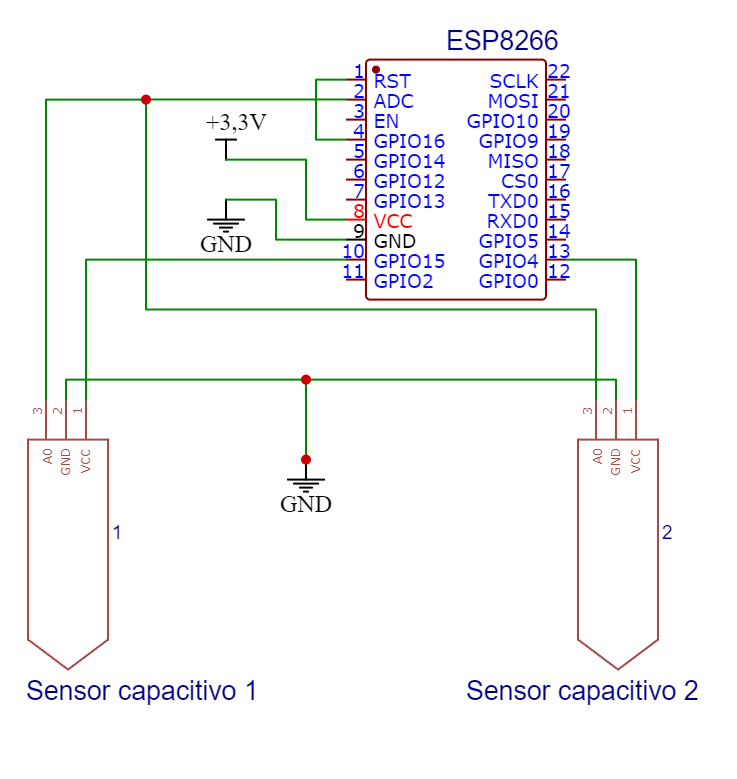
\includegraphics[width=1\textwidth]{./Figures/soil_schem_doble.png}
		\caption[Módulo sensor doble]{Módulo sensor doble.}
		\label{fig:soilschem2}
     \end{subfigure}
     \hfill
        \caption[Esquema de conexión de módulos sensores de humedad del suelo]{Esquema de conexión de módulos sensores de humedad del suelo.}	\label{fig:soilschem}
\end{figure}
%\begin{figure}[!h]
%	\centering
%	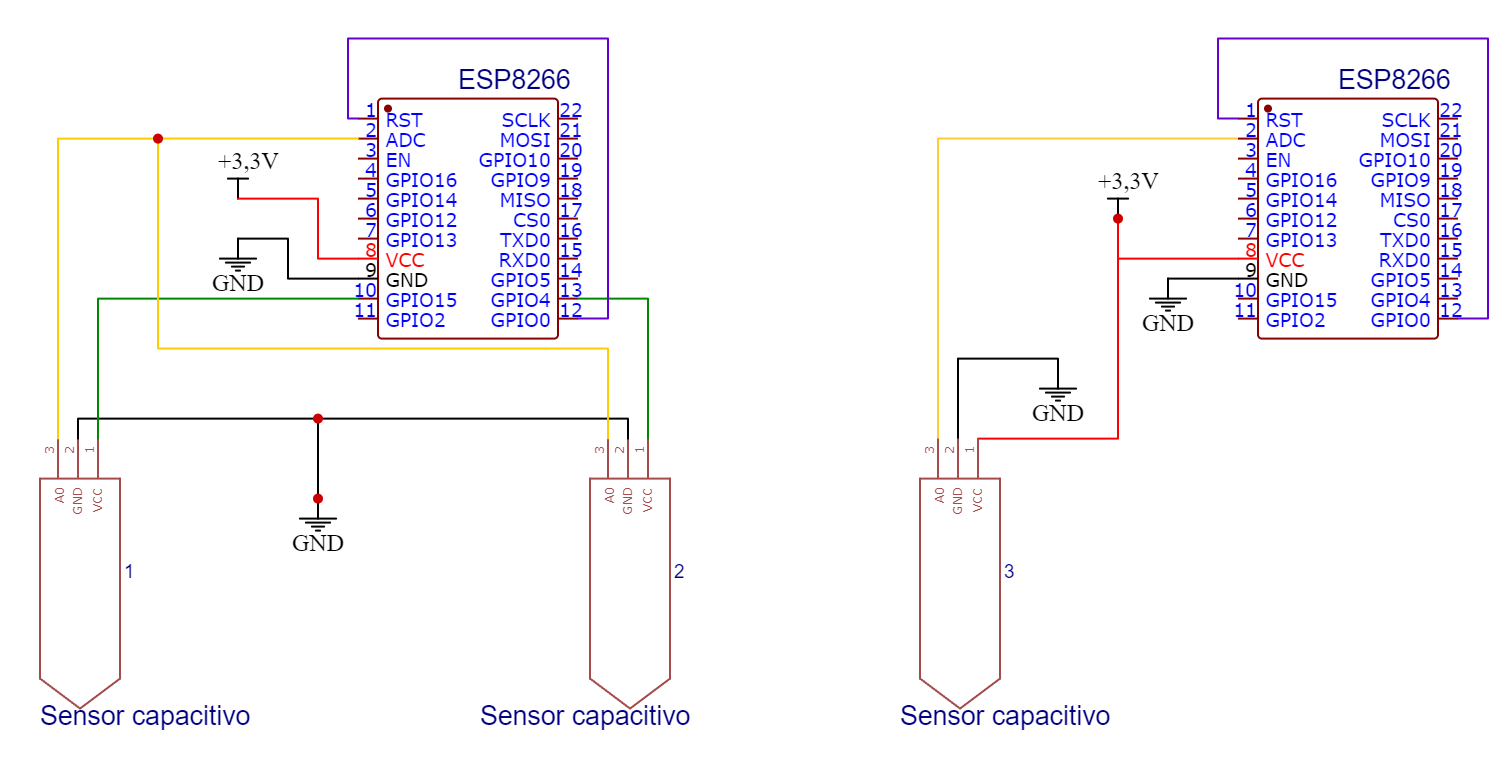
\includegraphics[width=1\textwidth]{./Figures/soil_schematic2.png}
%	\caption[Conexión del sensor de humedad del suelo]{Conexión del sensor de humedad del suelo.}
%	\label{fig:soilschem}
%\end{figure}

La integración de los componentes de los sensores se  realizó en forma manual por medio de placas de circuitos impresos (PCB) experimentales. En las figuras \ref{fig:soil1} y \ref{fig:soil2} se muestran los componentes empleados y un módulo ensamblado.

Dado que los sensores están expuestos a salpicaduras, se los recubrió con tubos adhesivos termocontraíbles que, al aplicarles calor, generan una protección a prueba de agua. Para el resguardo del chip ESP8266 se utilizó una caja de polipropileno transparente sellada. En las figuras \ref{fig:soil3} y \ref{fig:soil4} se muestran los componentes y sus protecciones. 

\begin{figure}[!h]
     \centering
     \begin{subfigure}[b]{0.45\textwidth}
		\centering
		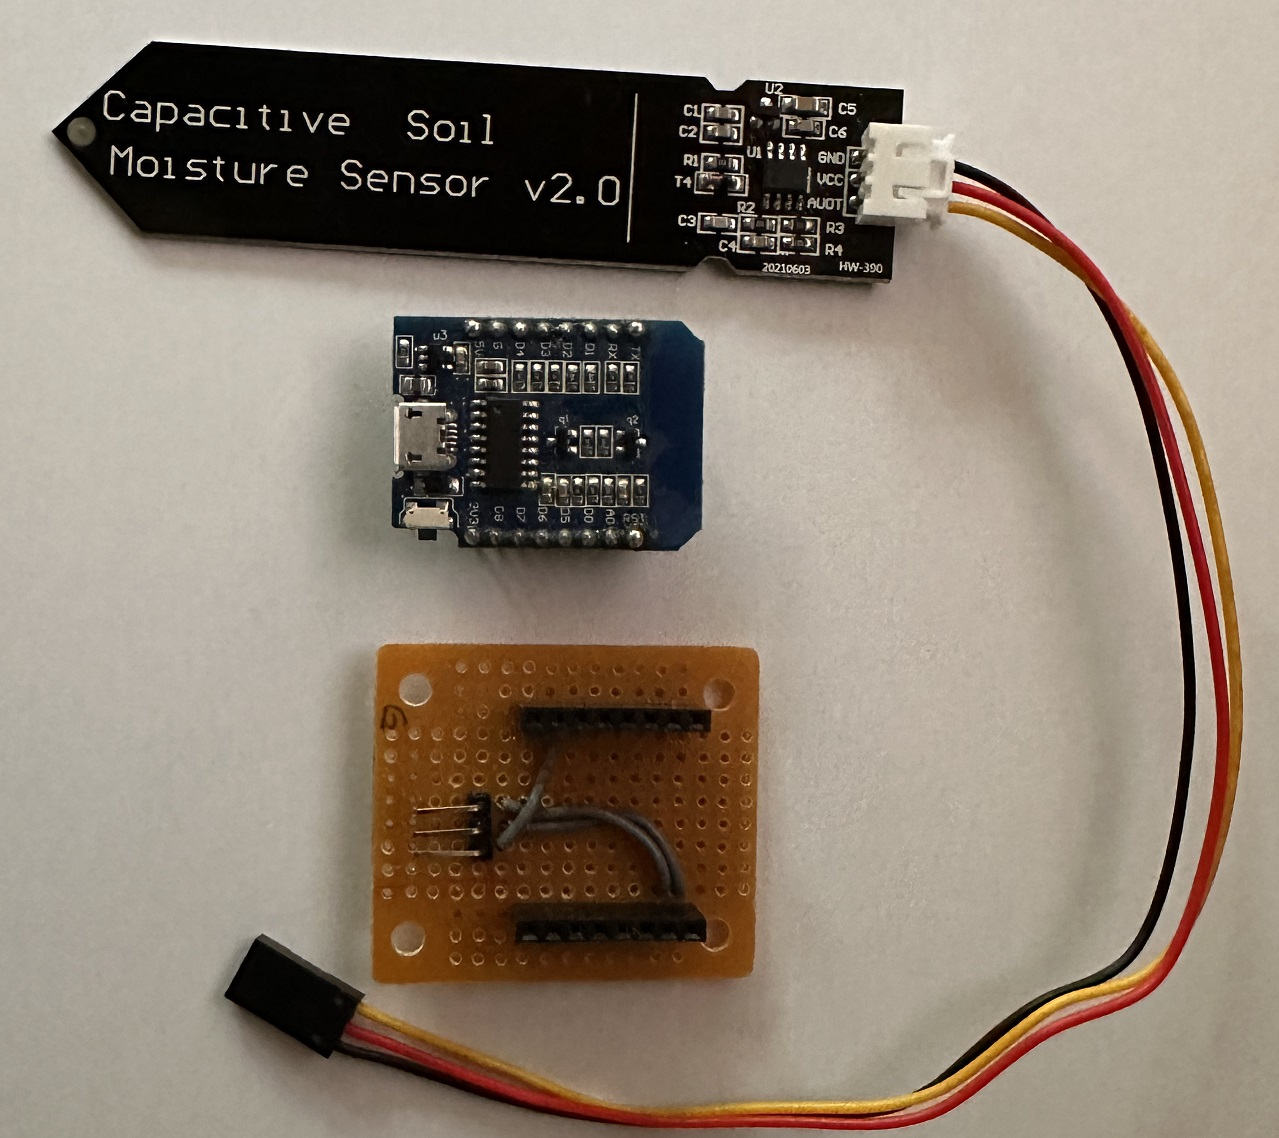
\includegraphics[width=0.80\textwidth]{./Figures/soil1.jpeg}
		\caption[Módulo con un sensor de humedad del suelo]{Módulo con un sensor de humedad del suelo.}
		\label{fig:soil1}
     \end{subfigure}
     \hfill
     \begin{subfigure}[b]{0.45\textwidth}
	\centering
		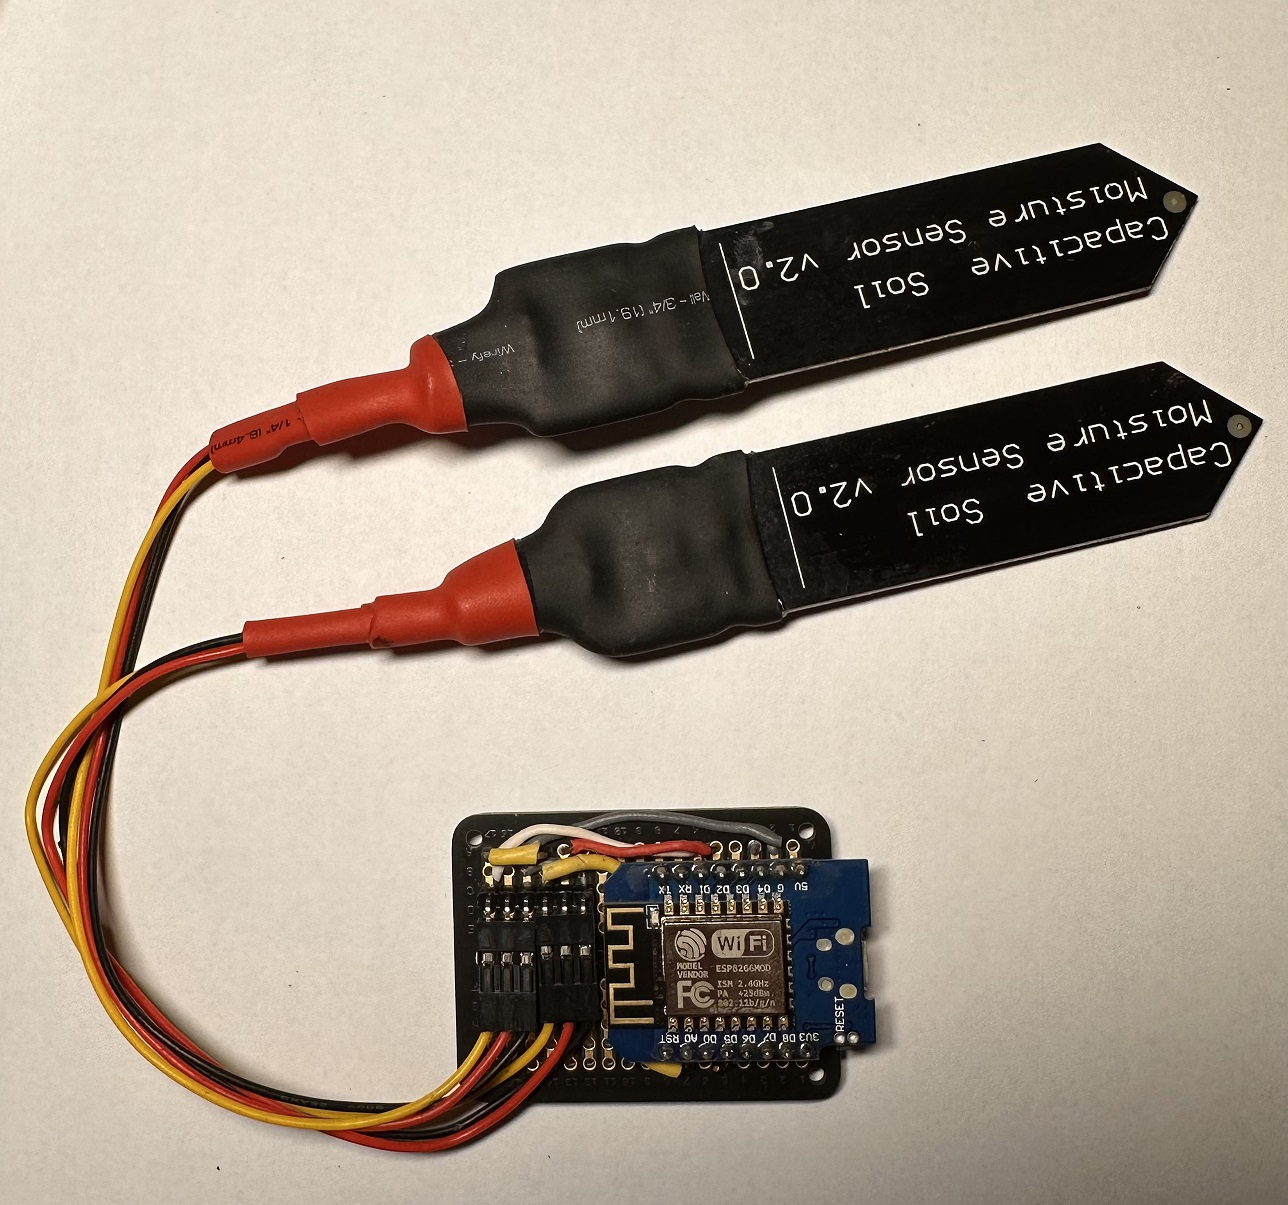
\includegraphics[width=0.80\textwidth]{./Figures/soil2.jpeg}
		\caption[Módulo con dos sensores de humedad del suelo]{Módulo con dos sensores de humedad del suelo.}
		\label{fig:soil2}
     \end{subfigure}
      \begin{subfigure}[b]{0.45\textwidth}
	\centering
		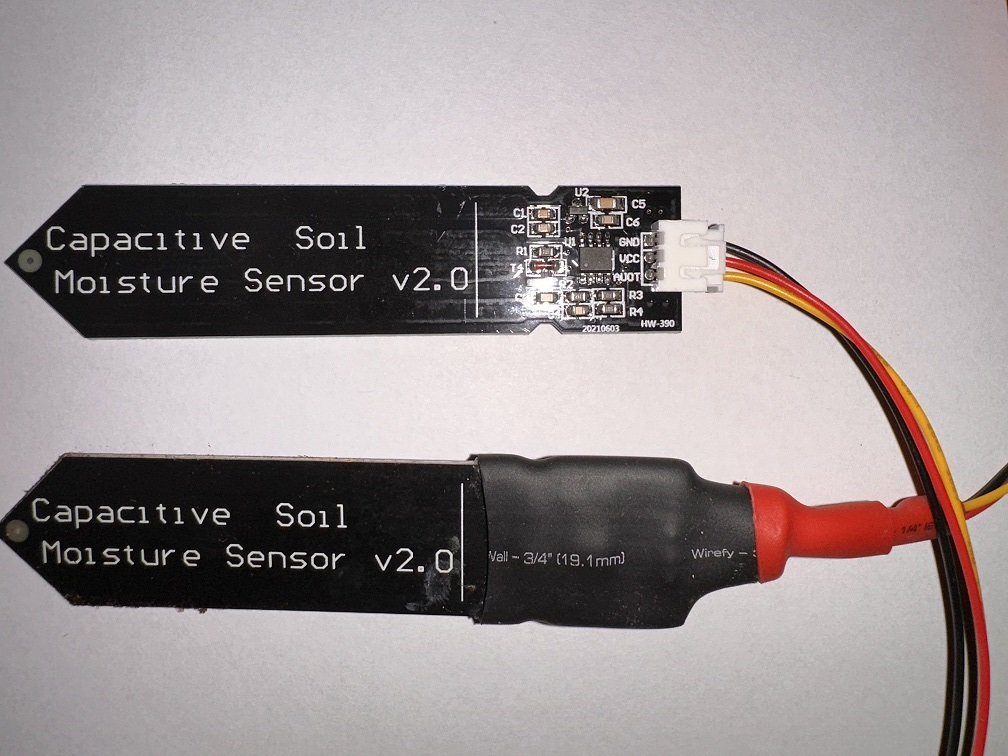
\includegraphics[width=0.80\textwidth]{./Figures/soil_compare.jpg}
		\caption[Detalle de protección de circuitos en los sensores]{Detalle de protección de circuitos en los sensores.}
		\label{fig:soil3}
     \end{subfigure}	
			\begin{subfigure}[b]{0.45\textwidth}
	\centering
		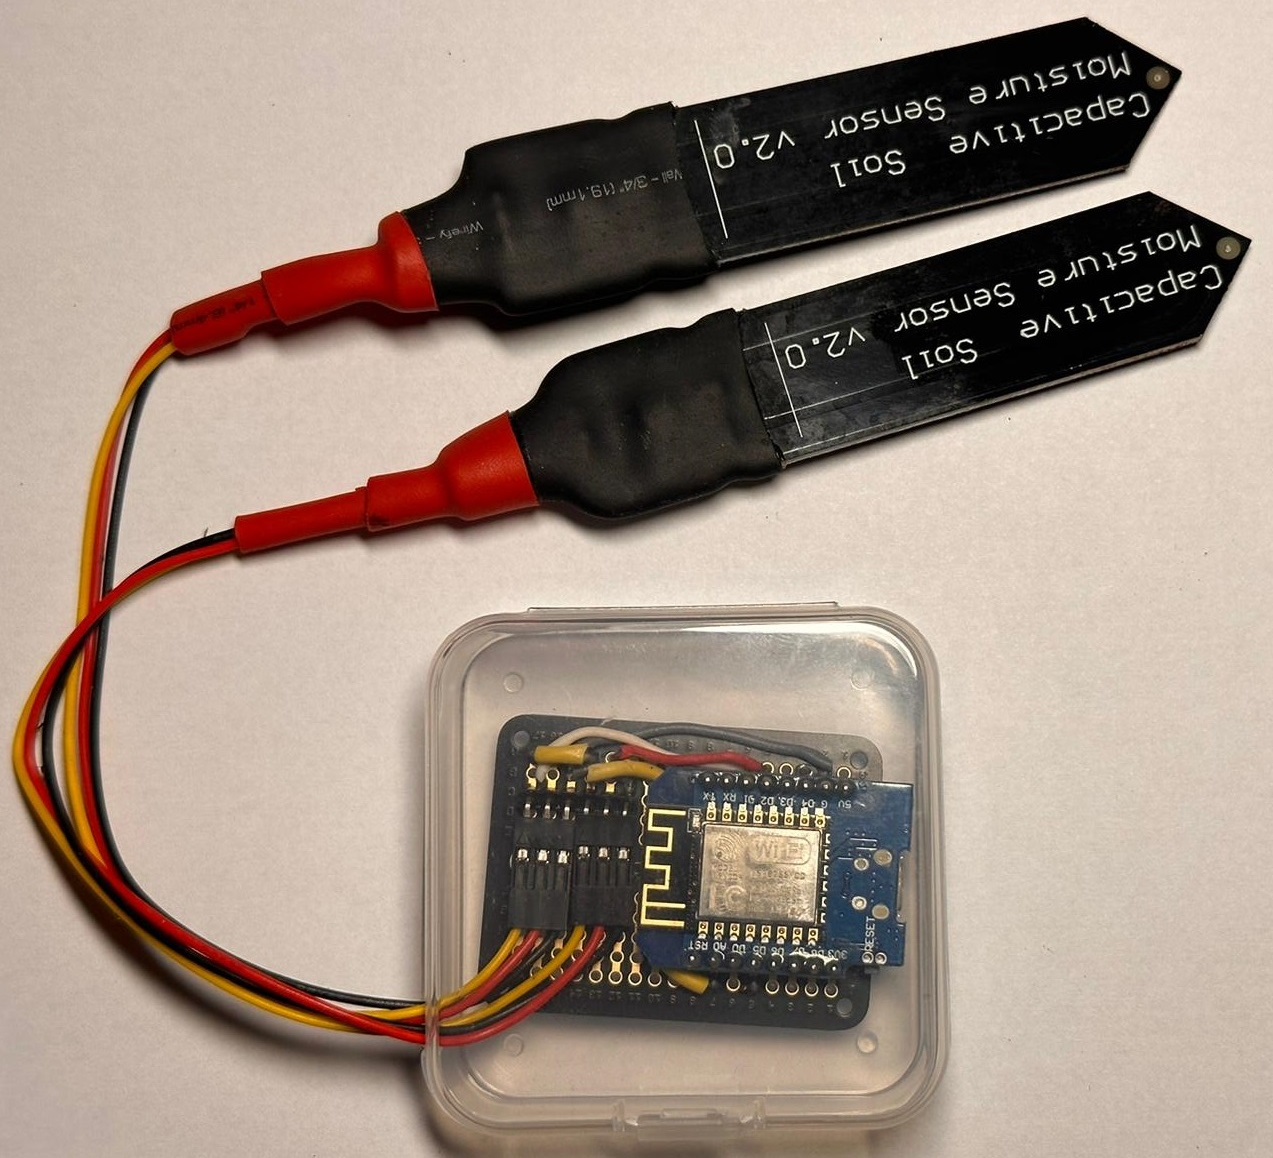
\includegraphics[width=0.80\textwidth]{./Figures/soil3.jpg}
		\caption[Módulo en su caja protectora]{Módulo en su caja protectora.}
		\label{fig:soil4}
     \end{subfigure}
     \hfill
        \caption[Módulos de sensores de humedad del suelo  empleados en el proyecto]{Módulo de sensores de humedad del suelo  empleados en el proyecto.}
        \label{fig:soilsenors}
\end{figure}


\pagebreak

\subsection{Módulo controlador del riego}
\label{Módulo controlador del riego}

Se compone de un microcontrolador ESP32, una placa de interfaz de relé de cuatro canales, una pantalla LCD/OLED SSH1106 y un regulador de voltaje DC-DC \textit{step down} LM2596. El esquema de conexiones entre estos componentes se detalla en la figura \ref{fig:riegochem}.

El módulo se alimenta con una fuente de 12 VDC y para energizar a los circuitos electrónicos el regulador LM2596 reduce la tensión a 5 VDC.

Para la construcción del prototipo se realizó la integración del microcontrolador con la pantalla LCD mediante una placa PCB experimental. Tanto para el módulo regulador de tensión como para el conjunto de relés se emplearon circuitos preensamblados. En la figura \ref{fig:riego_control} se muestran los componentes, su conexionado y la versión final de la unidad dentro de una caja protectora.   


\begin{figure}[!h]
	\centering
	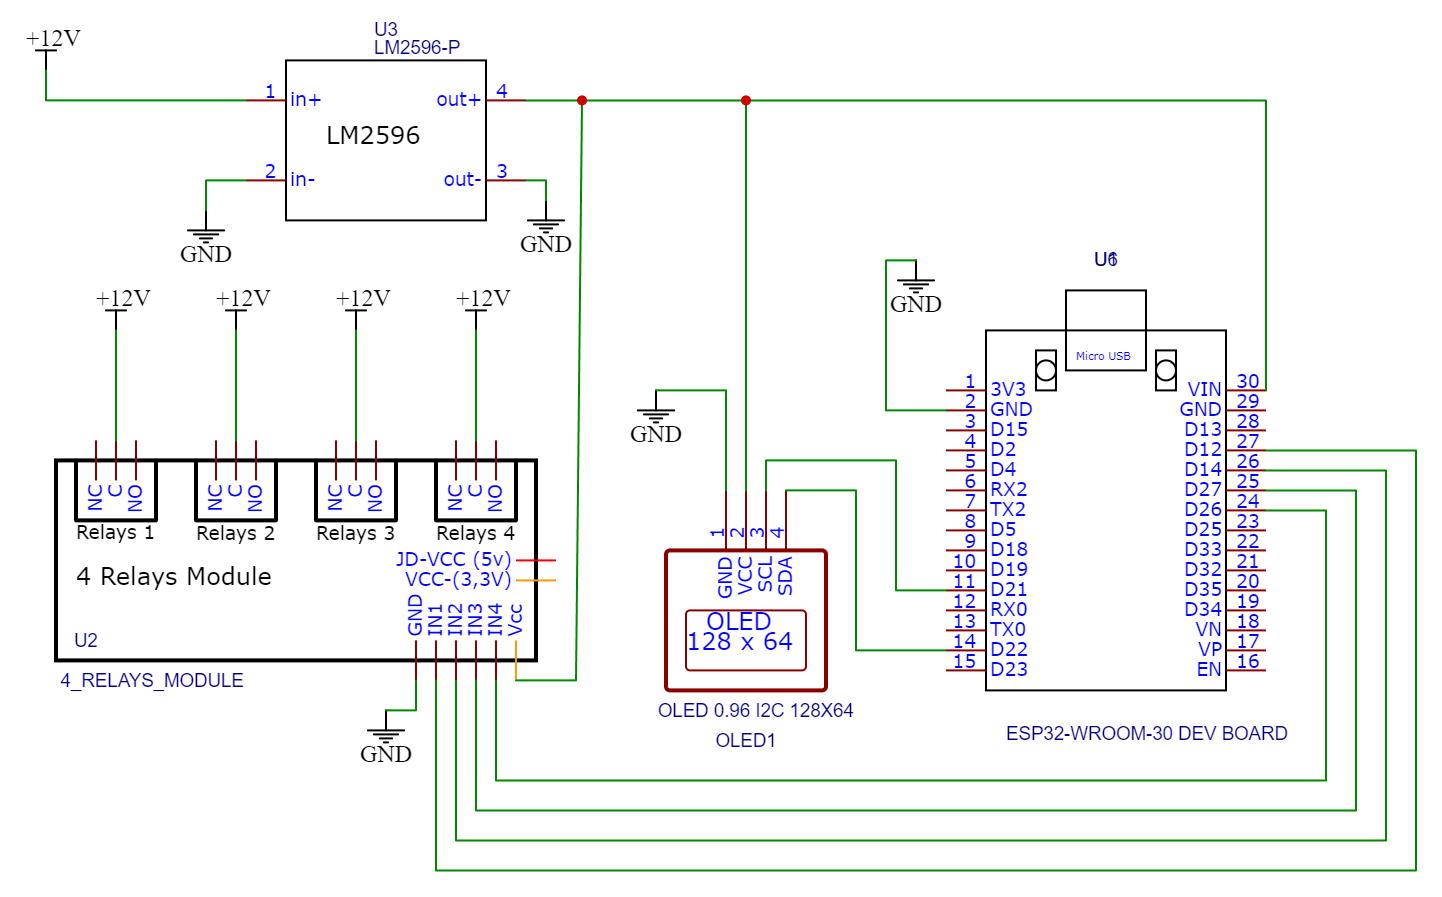
\includegraphics[width=0.9\textwidth]{./Figures/pump_schem.png}
	\caption[Conexión del módulo de control de riego]{Conexión del módulo de control de riego.}
	\label{fig:riegochem}
\end{figure}



\begin{figure}[!h]
     \centering
     \begin{subfigure}[b]{0.45\textwidth}
		\centering
		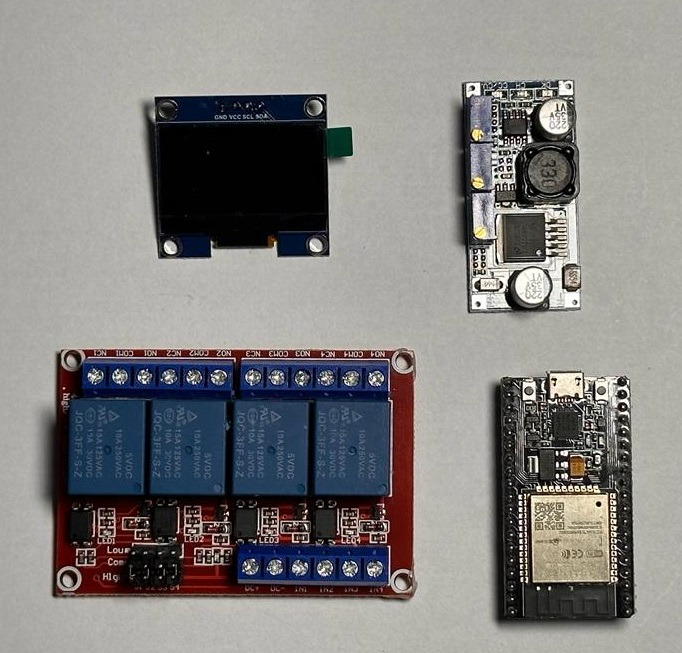
\includegraphics[width=0.8\textwidth]{./Figures/control_riego1.jpg}
		\caption[Detalle de los componentes]{Detalle de los componentes.}
		\label{fig:riego1}
     \end{subfigure}
     \hfill
     \begin{subfigure}[b]{0.45\textwidth}
	\centering
		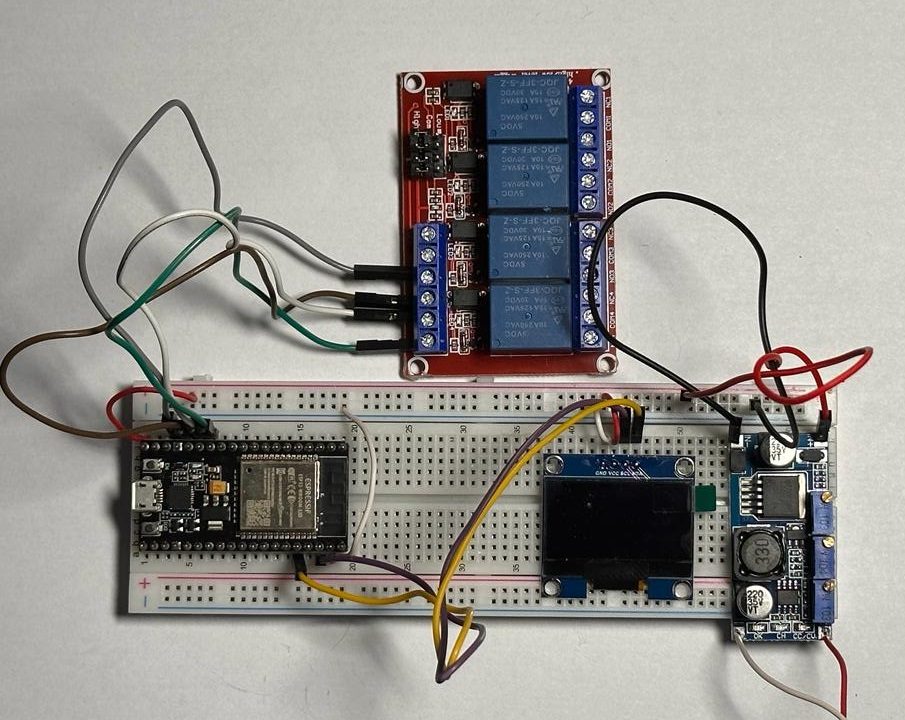
\includegraphics[width=1\textwidth]{./Figures/control_riego2.jpg}
		\caption[Conexionado]{Conexionado.}
		\label{fig:riego2}
     \end{subfigure}
      \begin{subfigure}[b]{0.45\textwidth}
	\centering
		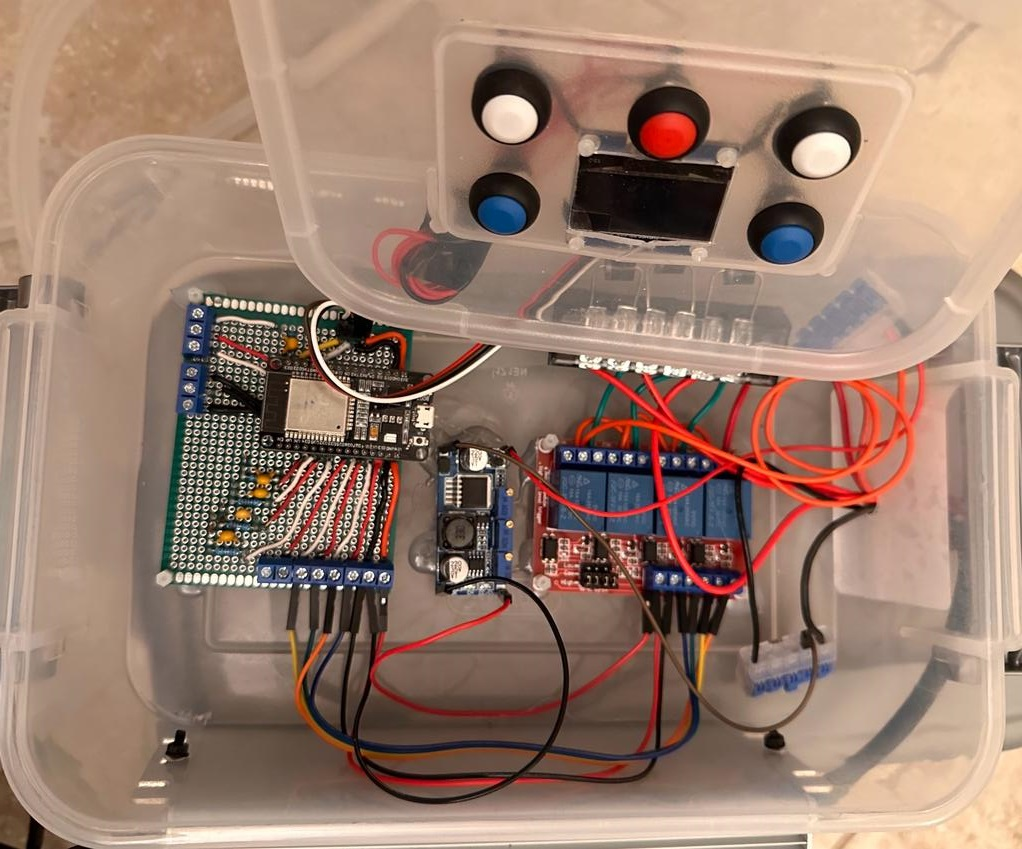
\includegraphics[width=0.8\textwidth]{./Figures/control_riego3.jpg}
		\caption[Conexionado]{Módulo finalizado en su caja protectora.}
		\label{fig:riego3}
     \end{subfigure}	
%			\begin{subfigure}[b]{0.45\textwidth}
%	\centering
%		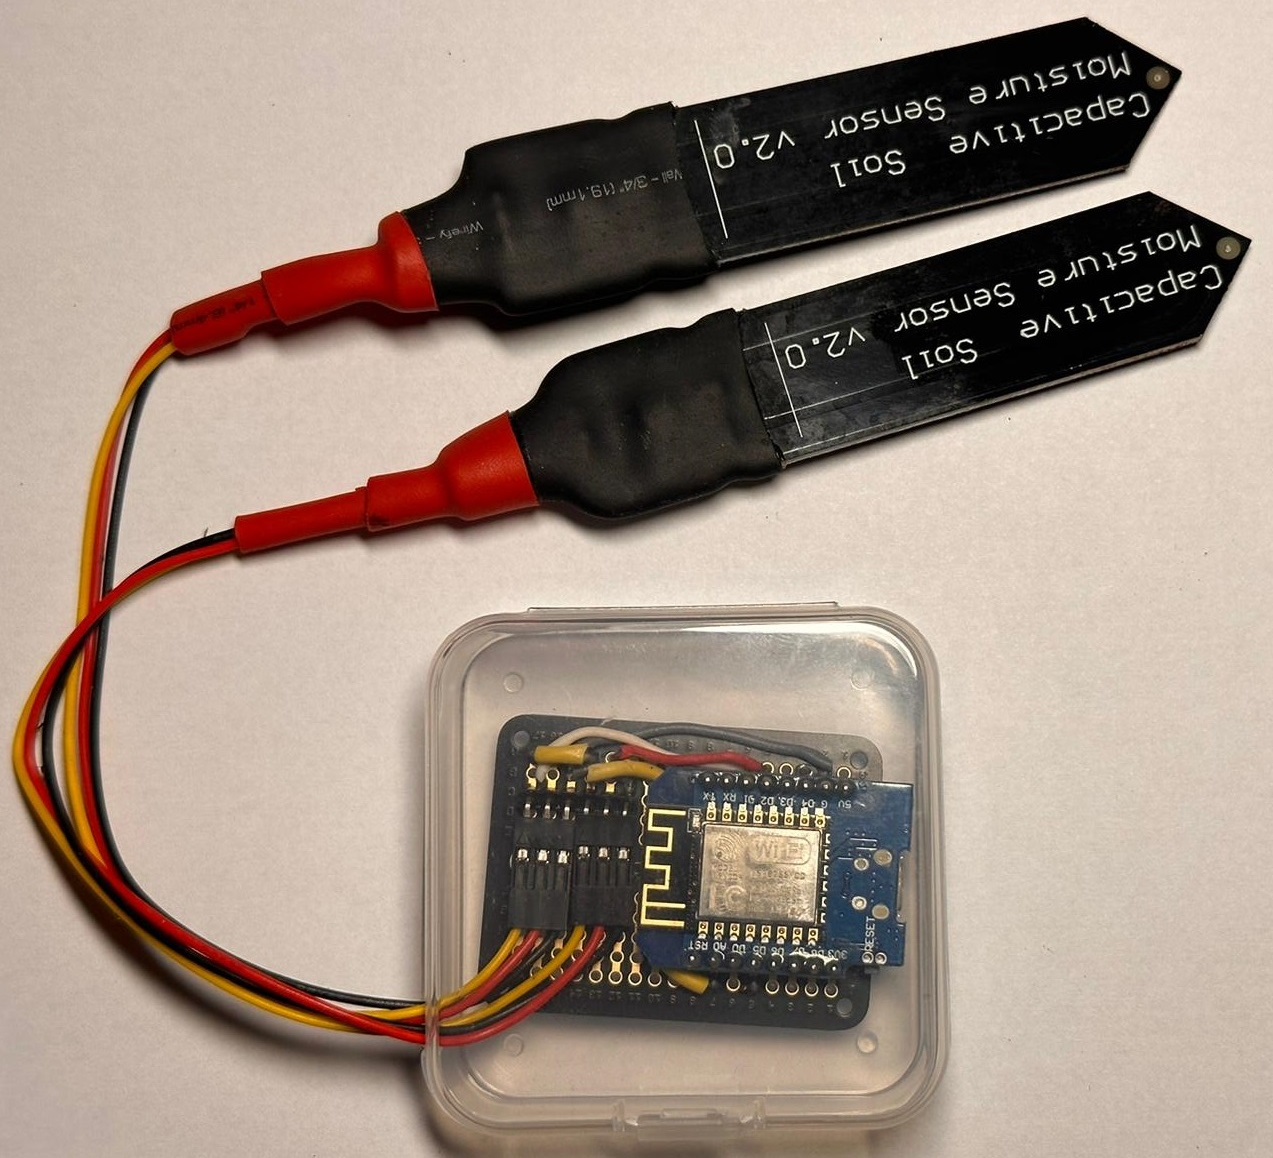
\includegraphics[width=0.60\textwidth]{./Figures/soil3.jpg}
%		\caption[Módulo en su caja protectora]{Módulo en su caja protectora.}
%		\label{fig:soil4}
%     \end{subfigure}
     \hfill
        \caption[Módulo de control de riego]{Módulo de control de riego.}
        \label{fig:riego_control}
\end{figure}


%\begin{figure}[!h]
%	\centering
%	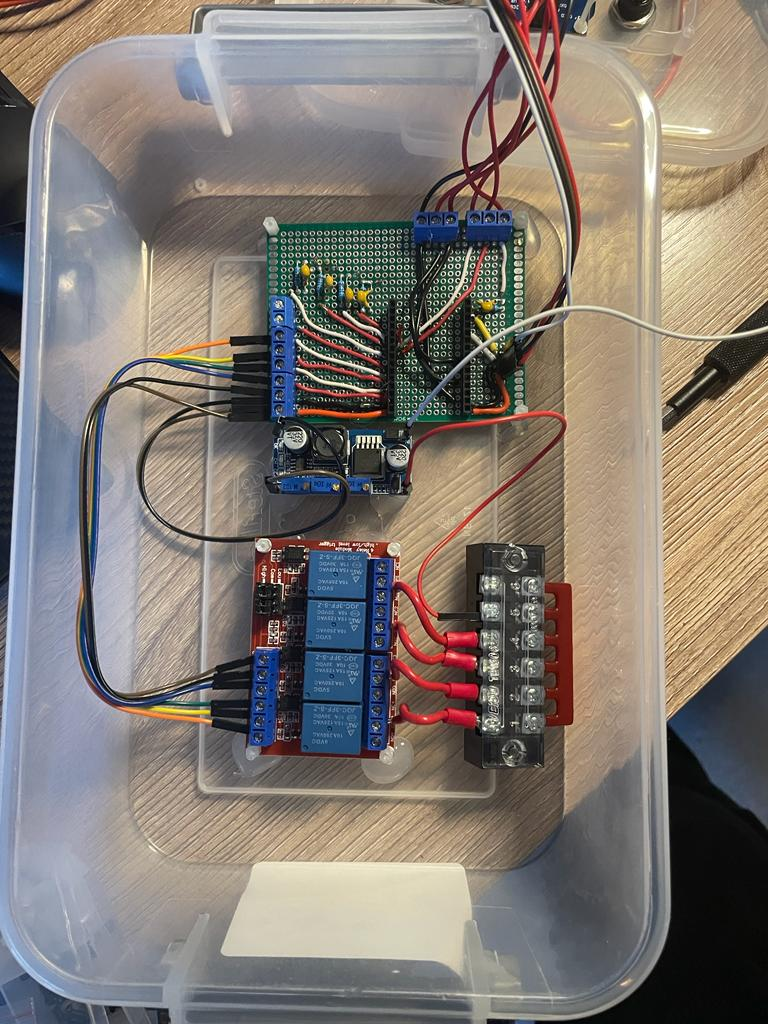
\includegraphics[width=0.5\textwidth]{./Figures/riego1.jpg}
%	\caption[Módulo completo en su caja protectora]{Módulo completo en su caja protectora.}
%	\label{fig:riego_control}
%\end{figure}
 
\pagebreak

\subsection{Módulo sensor de temperatura y humedad}
\label{Módulo sensor de temperatura y humedad}

Está compuesto por un microcontrolador ESP8266, un sensor DHT22 y una pantalla LCD/OLED SSH1106 para visualizar los valores de temperatura y humedad  \textit{in situ} en tiempo real. El esquema de conexión de los componentes se puede ver en la figura \ref{fig:tempschem}.

A diferencia de las sondas de humedad del suelo, el sensor de temperatura y humedad está pensado para instalarse en una ubicación fija 
con acceso a la red eléctrica. Por este motivo no se consideró configurarlo para soportar \textit{deep sleep}.



La construcción del módulo se realizó sobre placa PCB experimental en forma similar a los demás sistemas.
Para proteger los componentes se utilizó una caja de polipropileno transparente. El sensor DHT22 quedó expuesto para medir las condiciones ambientales como muestra la figura \ref{fig:temp_sensor}.


\begin{figure}[!h]
	\centering
	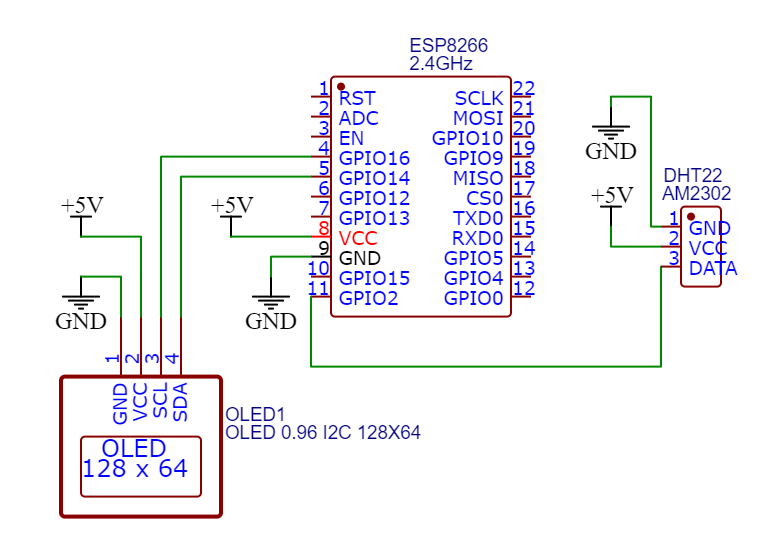
\includegraphics[width=0.7\textwidth]{./Figures/temp_sensor.png}
	\caption[Conexión del sensor de temperatura y humedad]{Conexión del sensor de temperatura y humedad.}
	\label{fig:tempschem}
\end{figure}


\begin{figure}[!h]
	\centering
	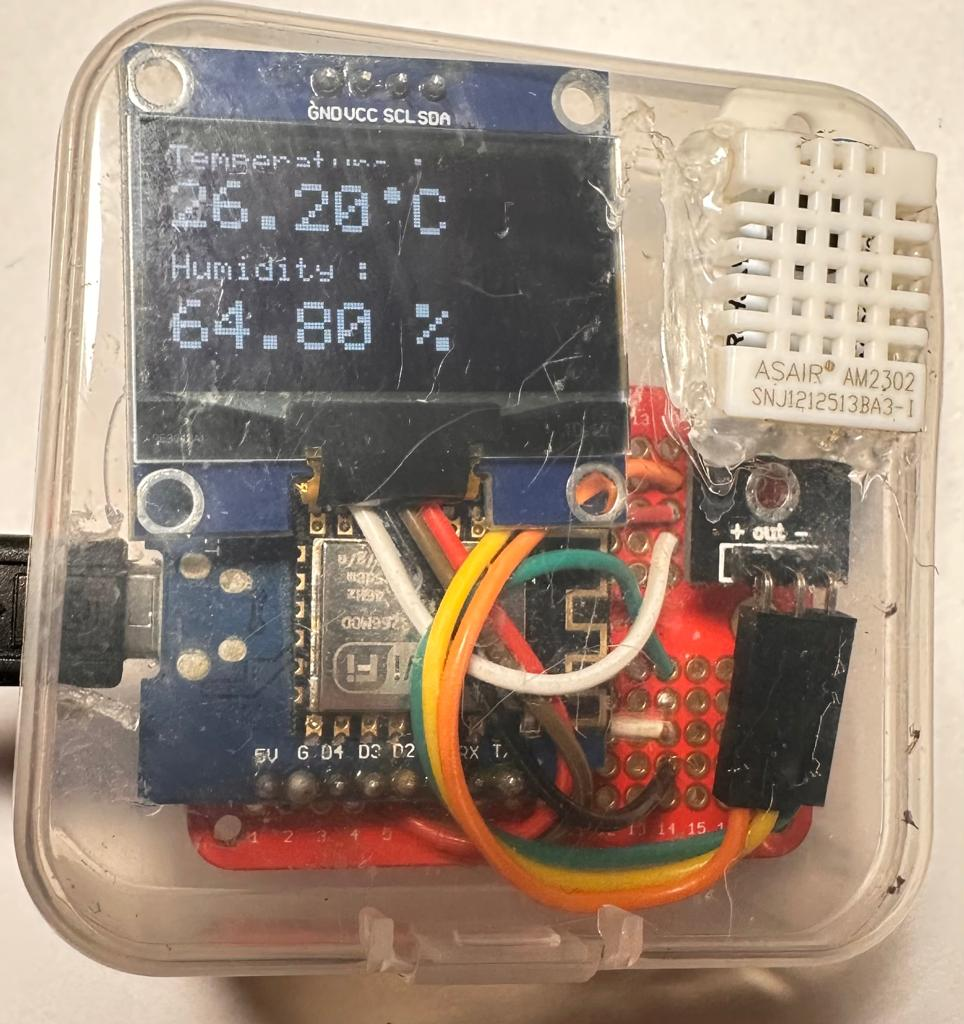
\includegraphics[width=0.5\textwidth]{./Figures/sensor_temp.jpg}
	\caption[Módulo completo en su caja protectora]{Módulo completo en su caja protectora.}
	\label{fig:temp_sensor}
\end{figure}


\subsection{Módulo controlador de clima}
\label{Módulo controlador de clima}

Es el responsable de accionar los ventiladores en el invernadero. Para el diseño se utilizó un chip ESP8266 conectado a un relé de una vía como se muestra en la figura \ref{fig:ventschem}. 

Dado que la salida del microcontrolador es de 3,3 V para el prototipo se seleccionó un relé que pueda ser accionado con ese valor de tensión, para evitar el uso de componentes adicionales tales como convertidores de tensión DC-DC \textit{step up}. 

En la figura \ref{fig:ventcontrol} se ilustra el proceso de construcción del módulo. 



\begin{figure}[!h]
	\centering
	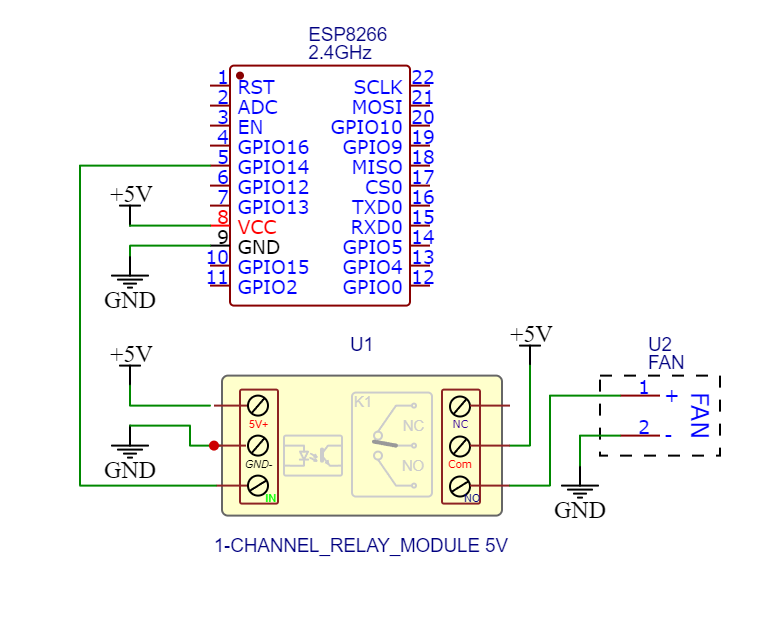
\includegraphics[width=0.7\textwidth]{./Figures/vent_schem.png}
	\caption[Conexión del módulo de control de clima]{Conexión del módulo de control de clima.}
	\label{fig:ventschem}
\end{figure}


\begin{figure}[!htpb]
     \centering
     \begin{subfigure}[b]{0.45\textwidth}
		\centering
		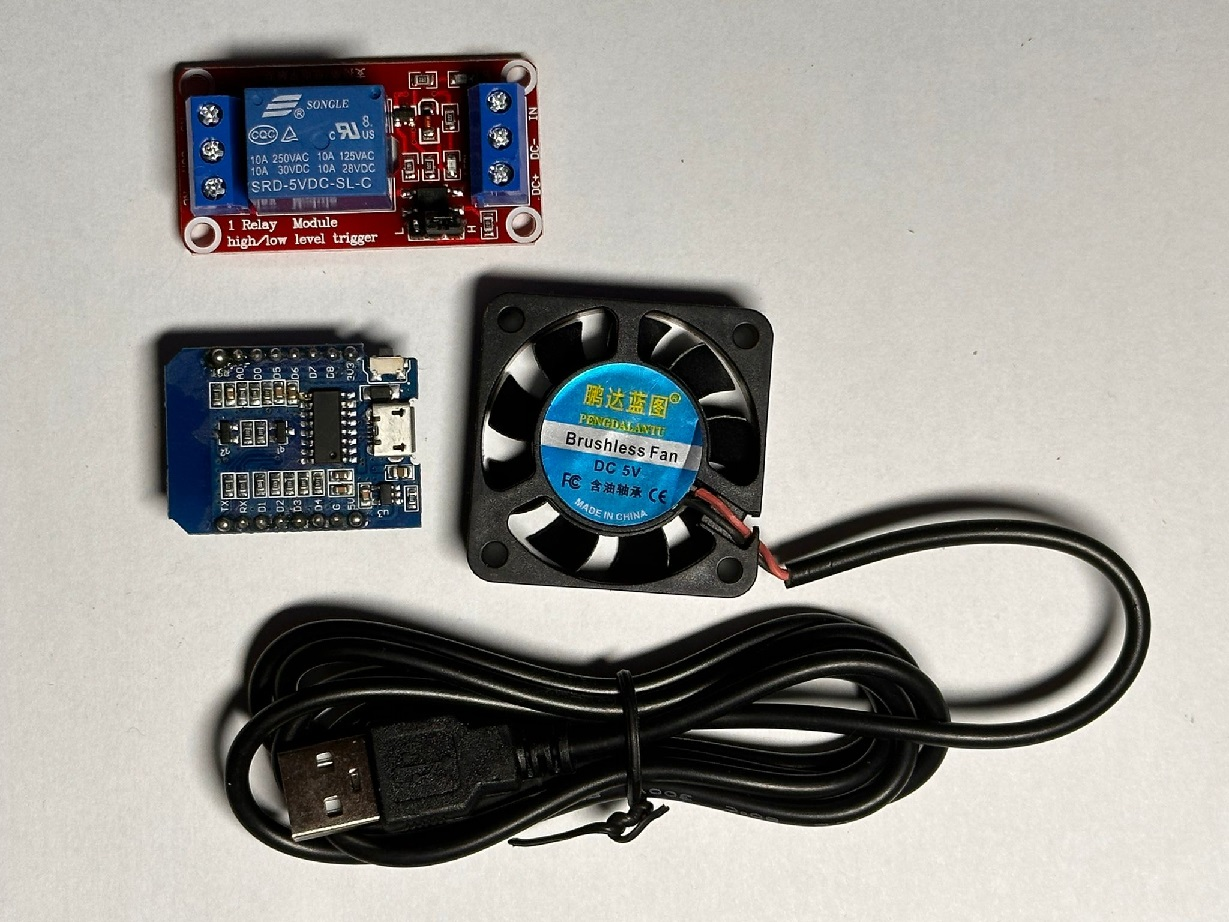
\includegraphics[width=0.80\textwidth]{./Figures/vent_control.jpg}
		\caption{Detalle de los componentes.}
		\label{fig:vent1}
     \end{subfigure}
     \hfill
     \begin{subfigure}[b]{0.45\textwidth}
	\centering
		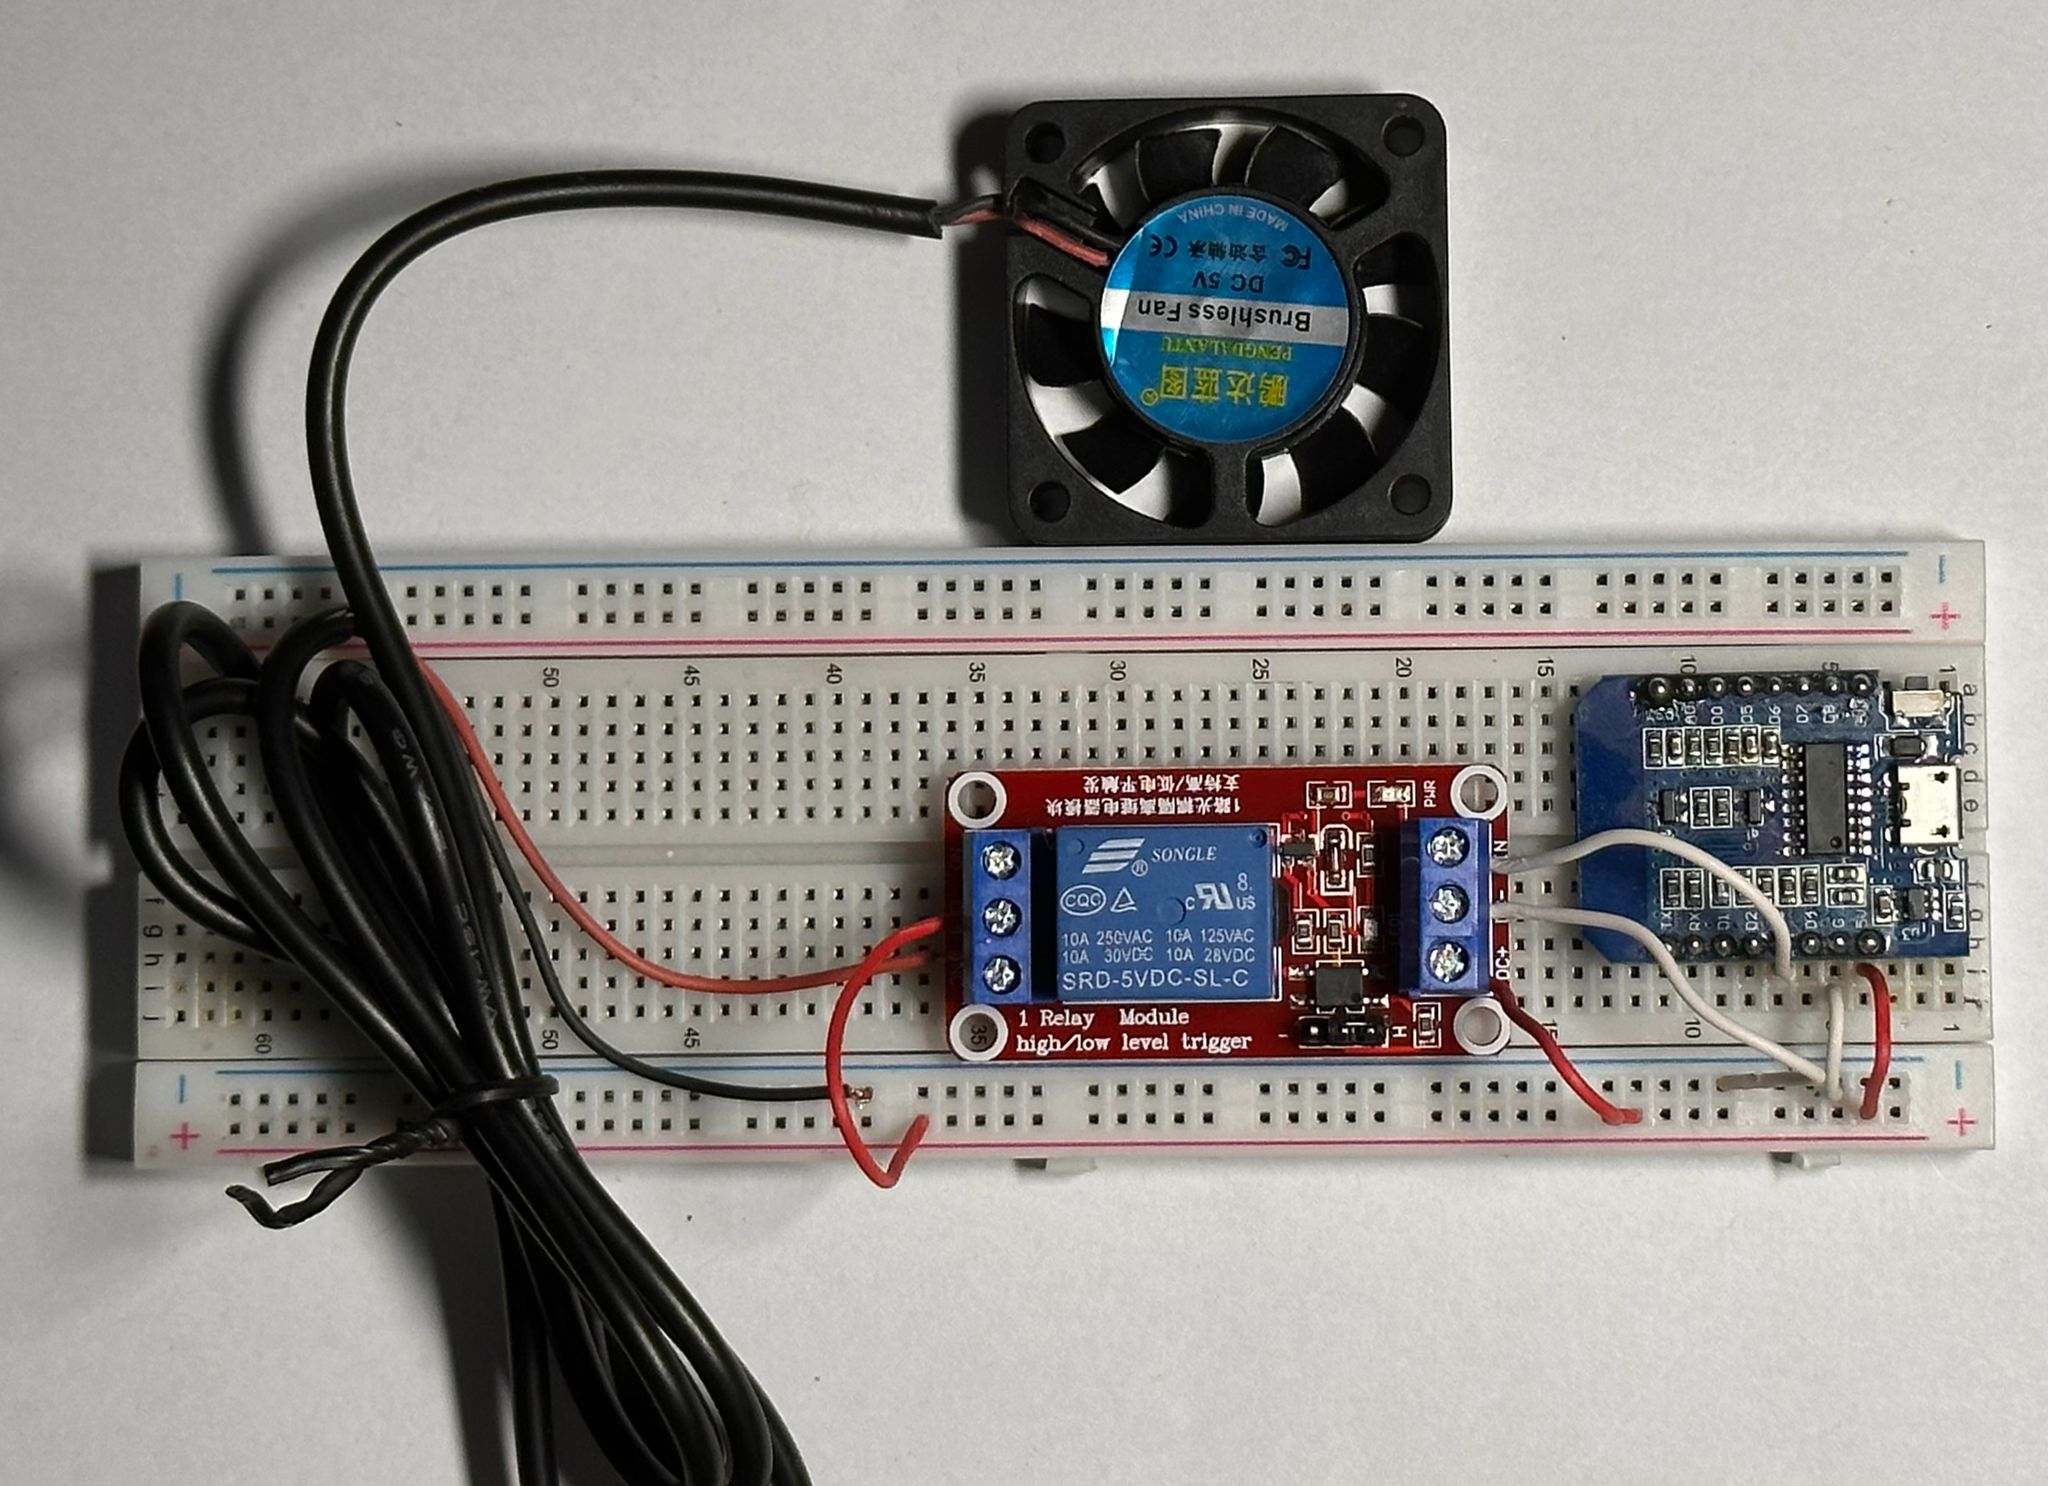
\includegraphics[width=0.80\textwidth]{./Figures/vent_proto.jpg}
		\caption{Conexionado.}
		\label{fig:vent2}
     \end{subfigure}	
	\begin{subfigure}[b]{0.45\textwidth}
		\centering
		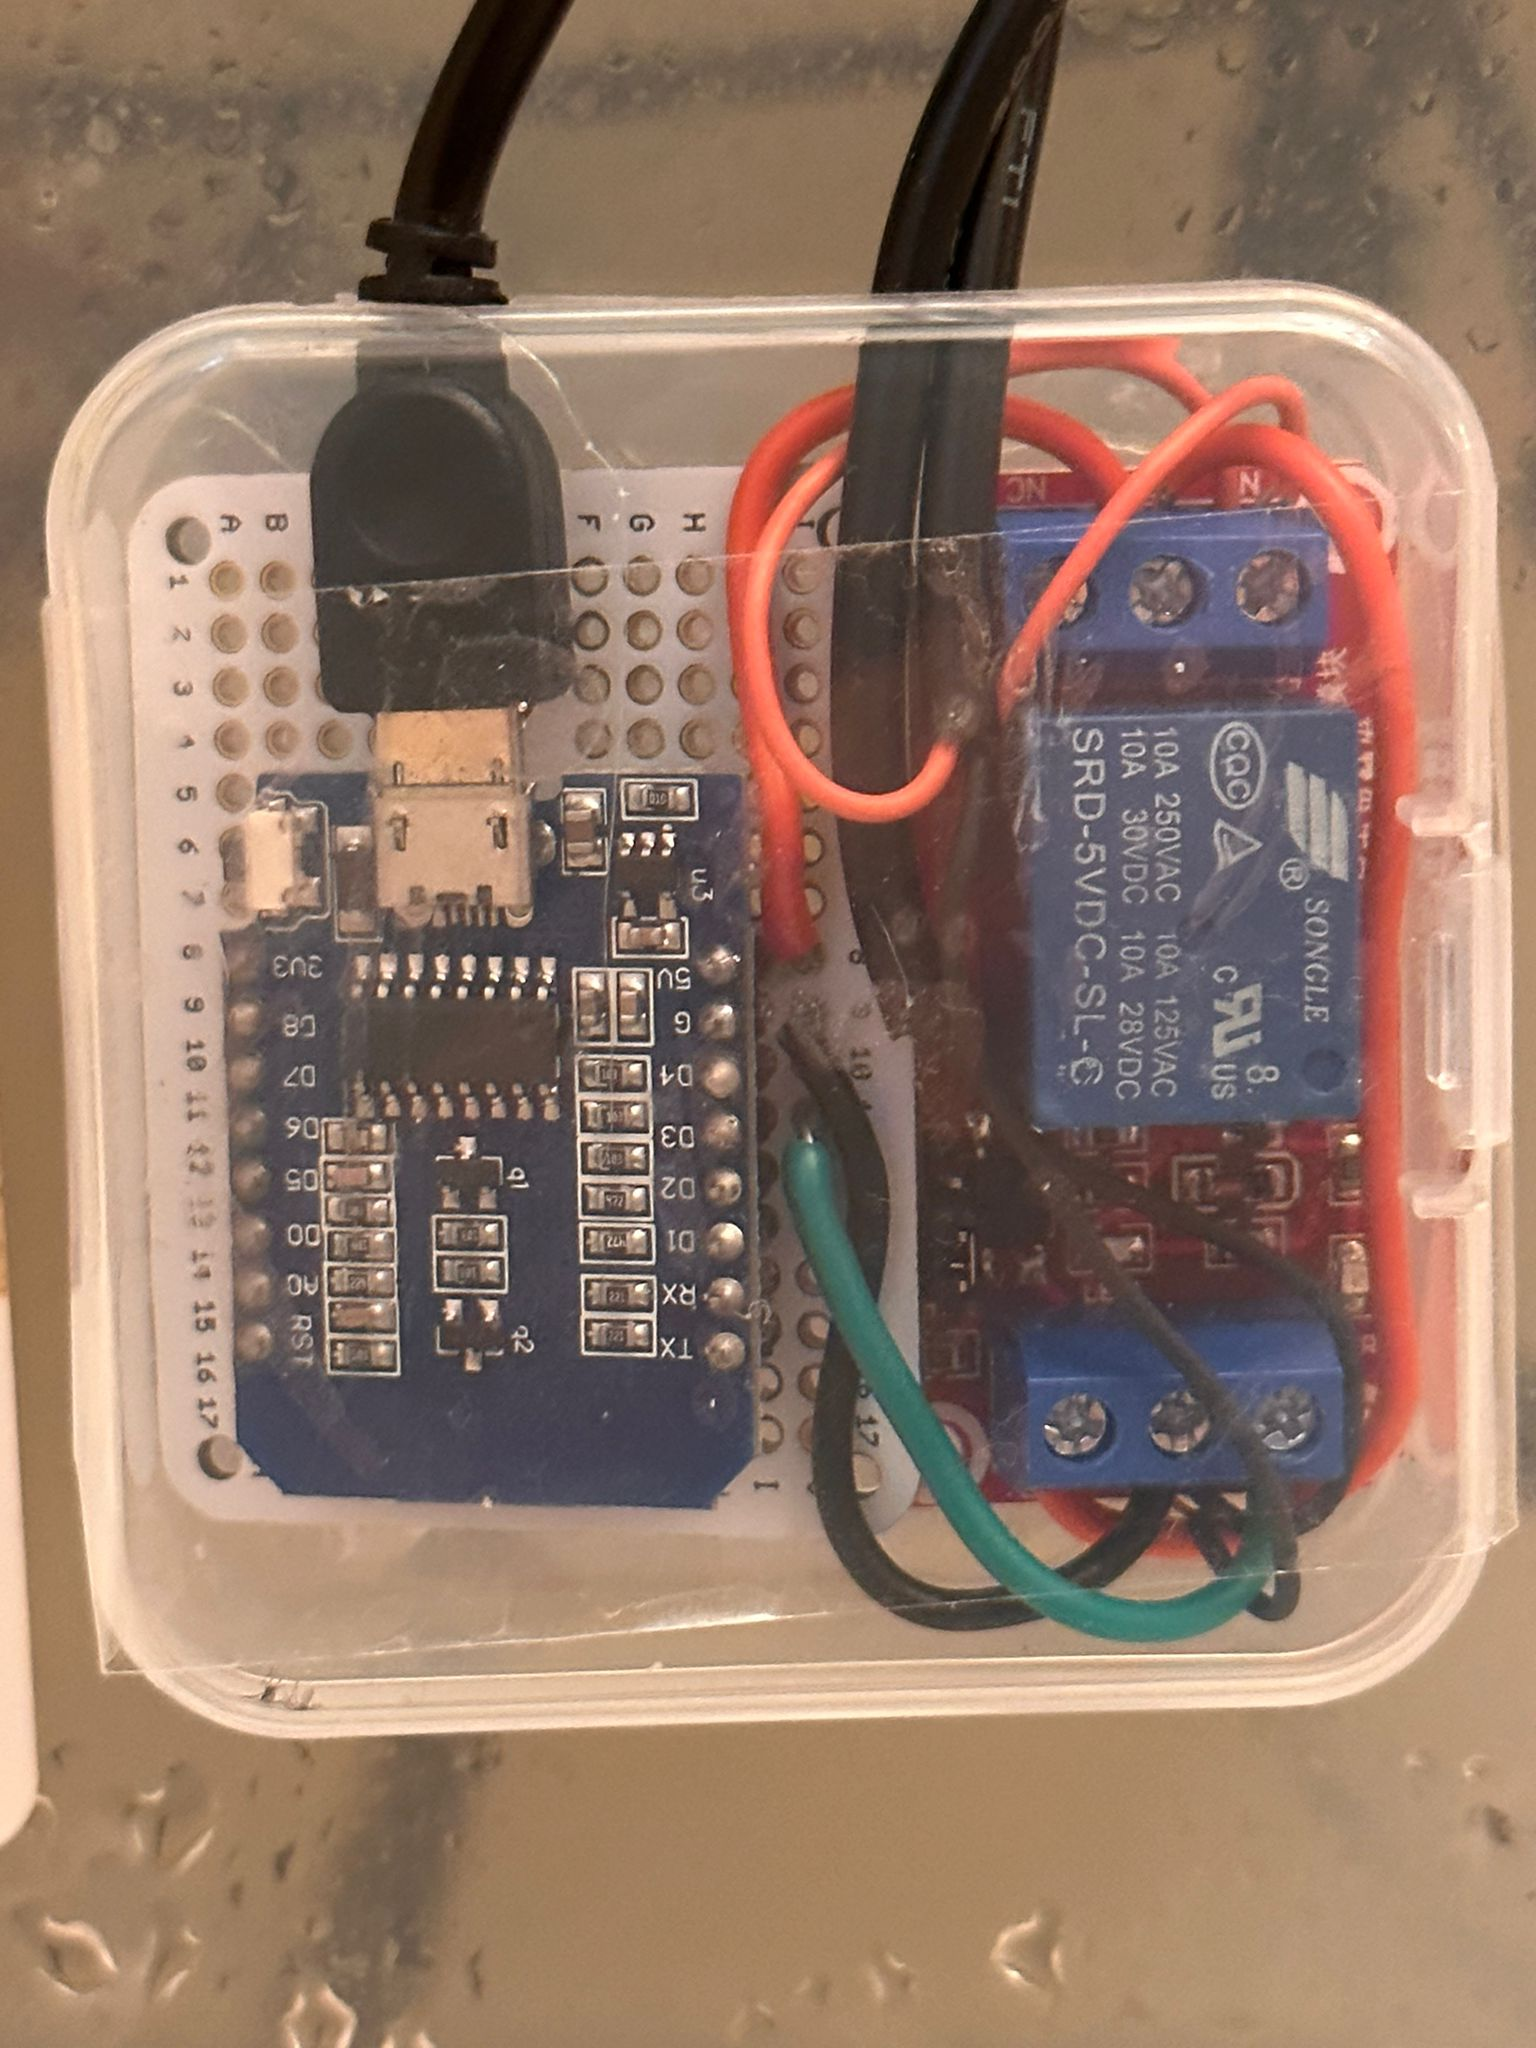
\includegraphics[width=0.60\textwidth]{./Figures/vent_assembled.jpg}
		\caption{Módulo finalizado en su caja protectora.}
		\label{fig:vent3}
     \end{subfigure}
     \hfill
        \caption[Módulo de control del clima]{Módulo de control del clima.}
        \label{fig:ventcontrol}
\end{figure}


\pagebreak

\section{Desarrollo del firmware}
\label{sec:Desarrollo del firmware}

Para la realización del proyecto se optó por desarrollar el firmware de todos los módulos en C++ por medio de la aplicación Arduino IDE. Los criterios utilizados para esta selección se basaron en la baja curva de aprendizaje de la herramienta, la amplia disponibilidad de librerías y ejemplos para el uso de componentes y la vasta comunidad de soporte para entusiastas de IoT existente en Internet.  Estos factores resultaron fundamentales para la elección debido a que el soporte y extensión del sistema quedará a cargo del cliente.

En líneas generales, el firmware de todos los módulos sigue el mismo patrón:

\begin{enumerate}
\item Comienzo: se corresponde al encendido del chip.
\item Setup: Es una función especial que se ejecuta una única vez al inicio del programa y se utiliza para inicializar cualquier variable, configurar los pines de entrada y salida y establecer cualquier comunicación que se precise.

\item Loop : Es una función que se ejecuta continuamente en un bucle que por lo general, solo se interrumpe al apagar al dispositivo. En esta sección se coloca el código principal del firmware.
\end{enumerate}
Adicionalmente, el código puede contener variables, funciones y bibliotecas.


Para facilitar la conexión a la aplicación Thingsboard, se hizo uso de la Arduino Thingsboard SDK \citep{tbsdk}, que provee mecanismos para el manejo de MQTT, RPC y provee la opción de realizar actualizaciones de firmware de forma inalámbrica (OTA de \textit{over the air}). 




\subsection{Firmware de los módulos sensores de humedad del suelo}
\label{Firmware de los módulos sensores de humedad del suelo}

Este es el único módulo que utiliza HTTP para la comunicación con la aplicación central debido a limitaciones en la aplicación Thignsboard, al no permitir configurar los períodos de retención de mensajes en las colas de MQTT para soportar configuraciones prolongadas de  \textit{deep sleep}. 

El proceso de ejecución es similar al resto, con la diferencia que luego del inicio, el programa realiza una llamada HTTP para obtener el tiempo de configuración de hibernación. La lectura de los sensores se realiza a continuación y varia de acuerdo a si es una configuración simple o doble. Esto es debido a que el ESP8266 posee un solo pin de conversión analógica a digital (ADC) al que todos las sondas deberán compartir. Para resolver este problema se procede a conectar la alimentación (VCC) de cada una de las sondas un pin GPIO diferente. De esta manera, al encender o apagar estos pines en forma secuencial, se energiza al sensor correspondiente y se procede a leer el valor en el pin ADC, para finalmente apagarlo y repetir el ciclo para el próximo sensor.

Para que el módulo pueda reportar un valor que represente la humedad del suelo, es necesario realizar una conversión del voltaje leído en el pin ADC. Se decidió seguir el método descripto en \citep{soilcalibration} que consiste en realizar mediciones en suelo seco para luego ir agregando cantidades precisas de agua sobre las que se evalúa la diferencia de potencial observada en cada caso. Del proceso resulta una fórmula lineal que calcula el contenido volumétrico de agua presente en la tierra.

Una vez obtenido el o los valores se los reporta a la aplicación por medio una llamada HTTP POST, luego de lo cual el sensor comienza el período de \textit{deep sleep} por la cantidad de tiempo definida en el atributo leído en primera instancia.

En la figura \ref{fig:flow_soilsensor} se diagrama la ejecución del módulo.


\begin{figure}[!h]
	\centering
	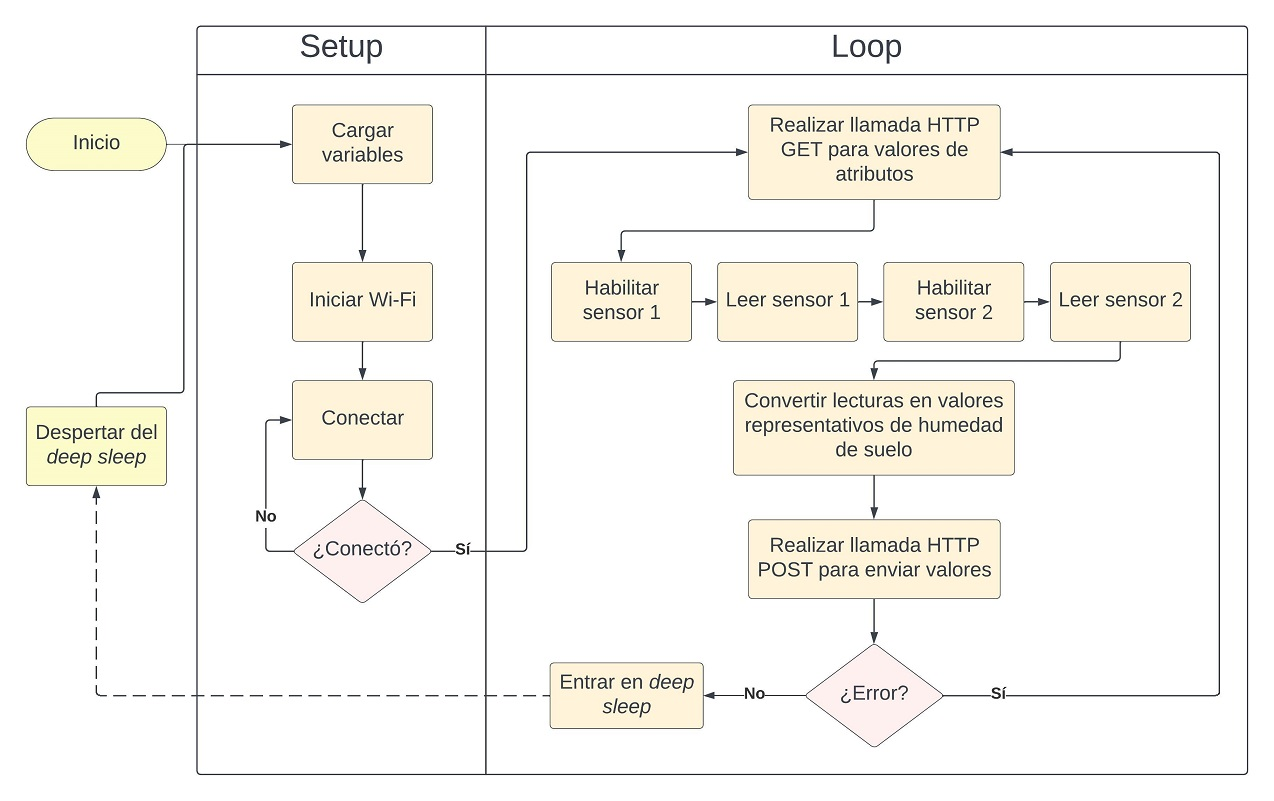
\includegraphics[width=0.9\textwidth]{./Figures/chapter3/FirmwareSoilSensor.jpg}
	\caption[Diagrama de flujo del firmware de los módulos sensores de humedad del suelo]{Diagrama de flujo del firmware de los módulos sensores de humedad del suelo.}
	\label{fig:flow_soilsensor}
\end{figure}


\pagebreak
\subsection{Firmware del módulo controlador del riego}
\label{Firmware del módulo controlador del riego}

Este es el módulo de mayor complejidad lo que puede verse reflejado en las figuras \ref{fig:flow_riegocontrol}, \ref{fig:flow_valvecontrol}  y \ref{fig:flow_bombacontrol}.

La ejecución se inicializa con el proceso estándar de carga de variables, entre las que se incluye un valor por defecto para la duración del riego, y el estado de la bomba y cada válvula presente. Luego de la conexión a la red Wi-Fi, el programa se registra a la aplicación y se subscribe a los \textit{getter topics} y a los  \textit{setter topics}, que se corresponden a los canales para reportar los estados a la aplicación o recibir comandos para prender o apagar dispositivos respectivamente.

En el caso de recibir un mensaje para informar el estado de los pines de GPIO, asociados con las válvulas o la bomba, o de la variable de duración de riego, el código reporta sobre el \textit{topic} de respuesta el estado requerid. En cambio, si el mensaje recibido para realizar un cambio, puede suceder una de las siguientes situaciones: es para comenzar el riego, el programa realiza una serie de verificaciones para asegurar la integridad de la bomba y cañerías del sistema de riego:
\begin{itemize}
\item Pedido de reconfigurar el tiempo de riego: el código actualiza la variable y retorna la comienzo del bucle.

\item Pedido de apertura o cierre de válvula:
    \begin{itemize}
    \item Apertura: Se procede a abrir la válvula seleccionada y se comprueba si la bomba esta en estado de pedido de encendido (bomba lista), en cuyo caso se ordena el encendido de la bomba.
    \item Cierre: se realiza una comprobación si hay otras válvulas abiertas, de ser así se procede con el cierre. En caso de ser la última, se ordena el apagado de la bomba y por último se procede al cierre de válvula.
    
    \end{itemize}

\item Pedido de prendido o apagado de la bomba:
    \begin{itemize}
    \item Prendido: En el caso de haber una válvula abierta, se procede a encender la bomba por el tiempo que marque la variable de duración de riego, luego de lo cual se procede al apagado de la bomba y cierre de las válvulas, en ese orden. De no haber válvulas abiertas, se configura la variable de bomba lista en positivo, indicando que el riego fue pedido pero aún no están dadas las condiciones.
    \item Apagado: En el caso de pedir una interrupción en el riego, se ordena el apagado de la bomba y el cierre de las válvula.
    
    \end{itemize}



\end{itemize}


\begin{figure}[!h]
	\centering
	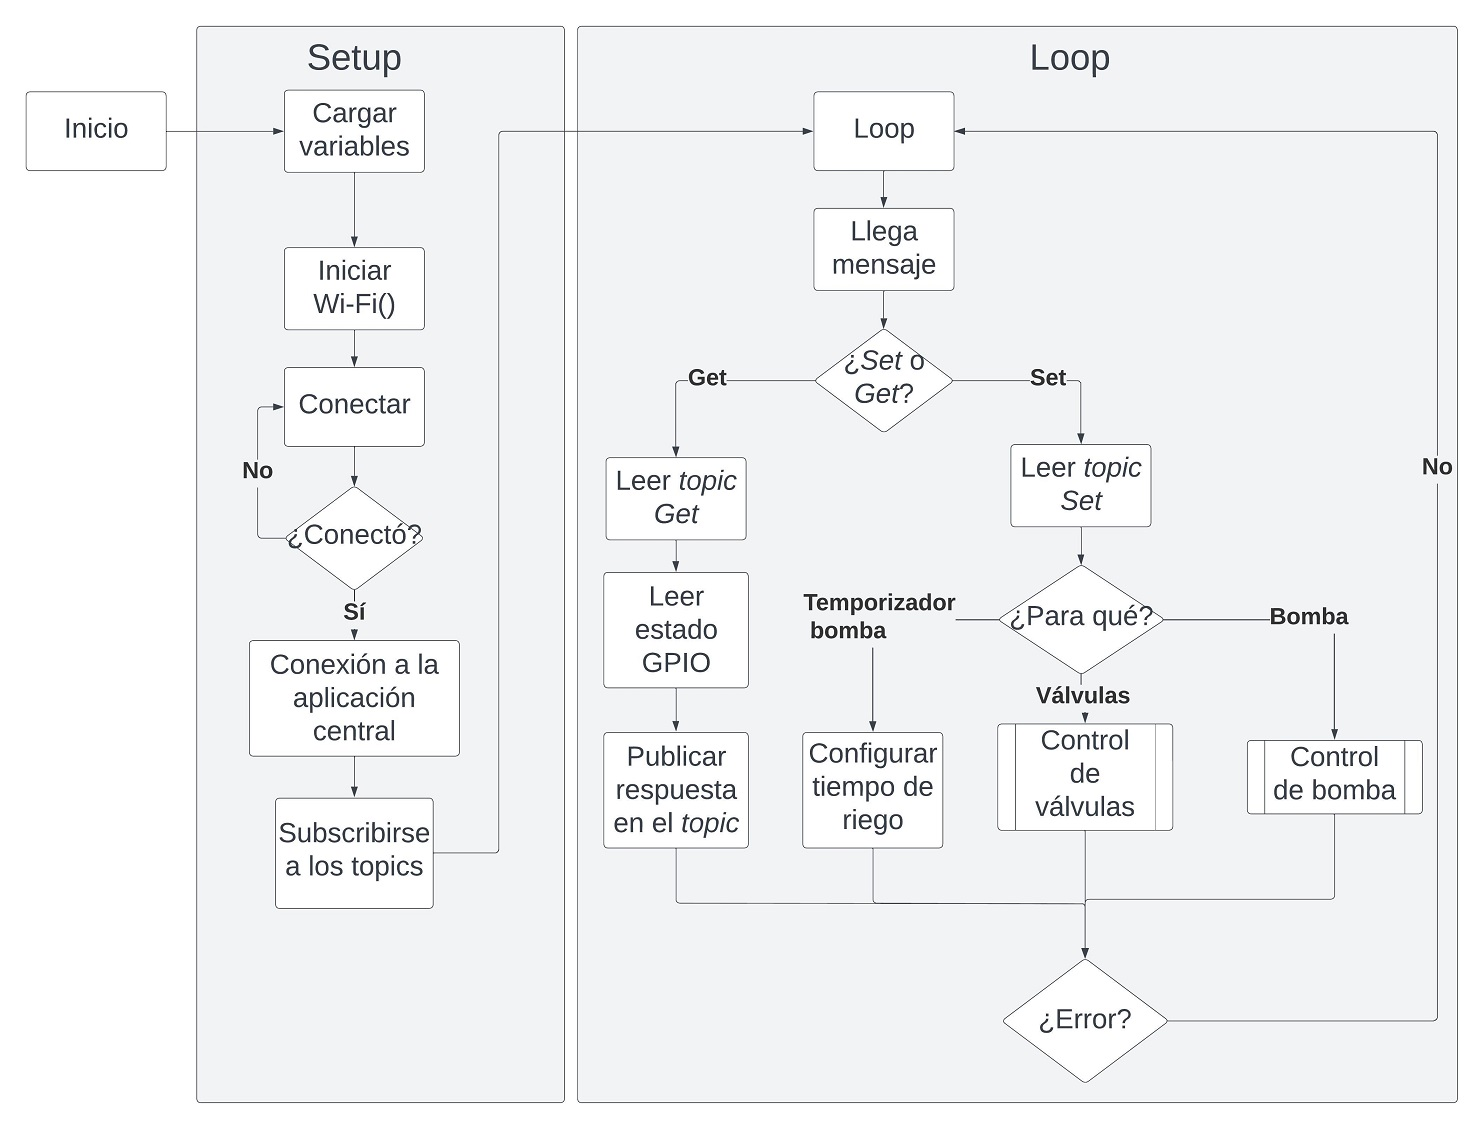
\includegraphics[width=0.9\textwidth]{./Figures/chapter3/FirmwareRiegoControl.jpg}
	\caption[Diagrama de flujo del firmware del módulo de control de riego]{Diagrama de flujo del firmware del módulo de control de riego.}
	\label{fig:flow_riegocontrol}
\end{figure}

\begin{figure}[!h]
	\centering
	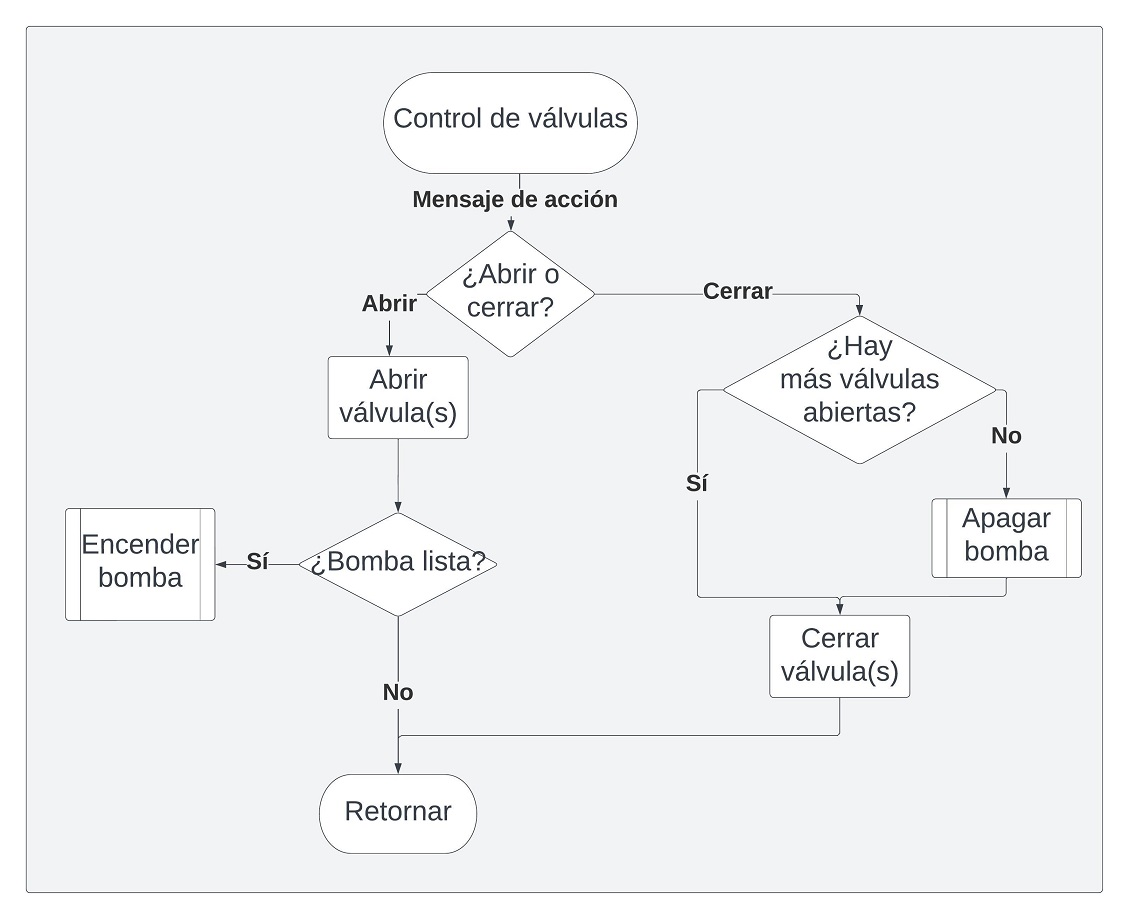
\includegraphics[width=0.7\textwidth]{./Figures/chapter3/FirmwareValveControl.jpg}
	\caption[Diagrama de flujo del firmware del módulo de control de riego - Control de válvulas]{Diagrama de flujo del firmware del módulo de control de riego - Control de válvulas.}
	\label{fig:flow_valvecontrol}
\end{figure}

\begin{figure}[!h]
	\centering
	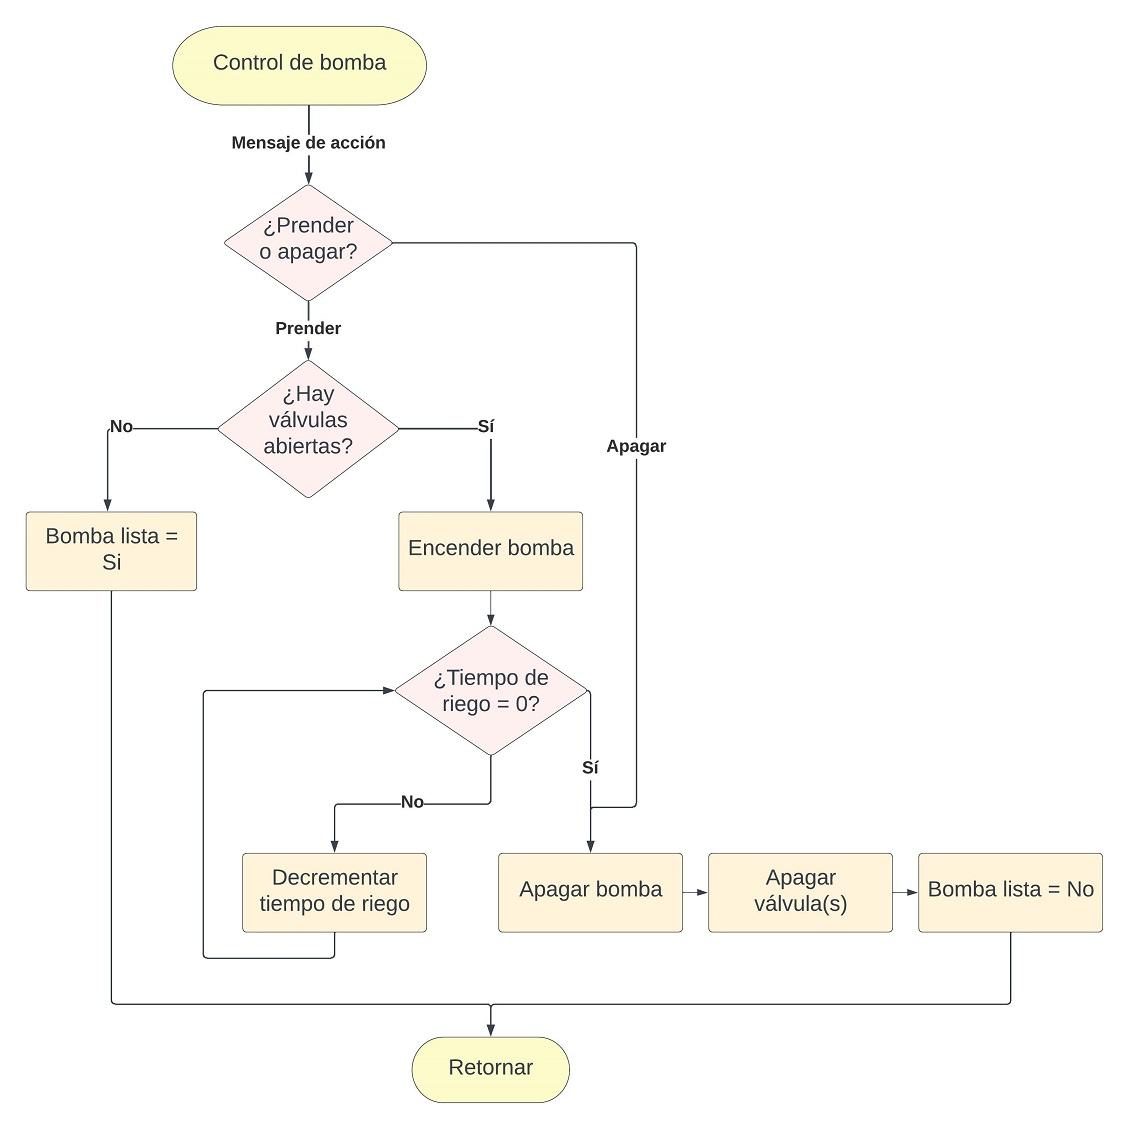
\includegraphics[width=0.7\textwidth]{./Figures/chapter3/FirmwarePumpControl.jpg}
	\caption[Diagrama de flujo del firmware del módulo de control de riego - Control de bomba]{Diagrama de flujo del firmware del módulo de control de riego - Control de bomba.}
	\label{fig:flow_bombacontrol}
\end{figure}







\pagebreak
\subsection{Firmware de los módulos sensores de temperatura y humedad}
\label{Firmware de los módulos sensores de de temperatura y humedad}

Se encarga de obtener las medidas de temperatura y humedad y reportarlas a la aplicación al mismo tiempo que imprime los valores en la pantalla LCD. Para reducir la cantidad de mensajes enviados, se incorpora un contador que indica cuántas iteraciones del ciclo son necesarias por cada envío de datos. Esto no se contempla para el reporte en la pantalla.


\begin{figure}[!h]
	\centering
	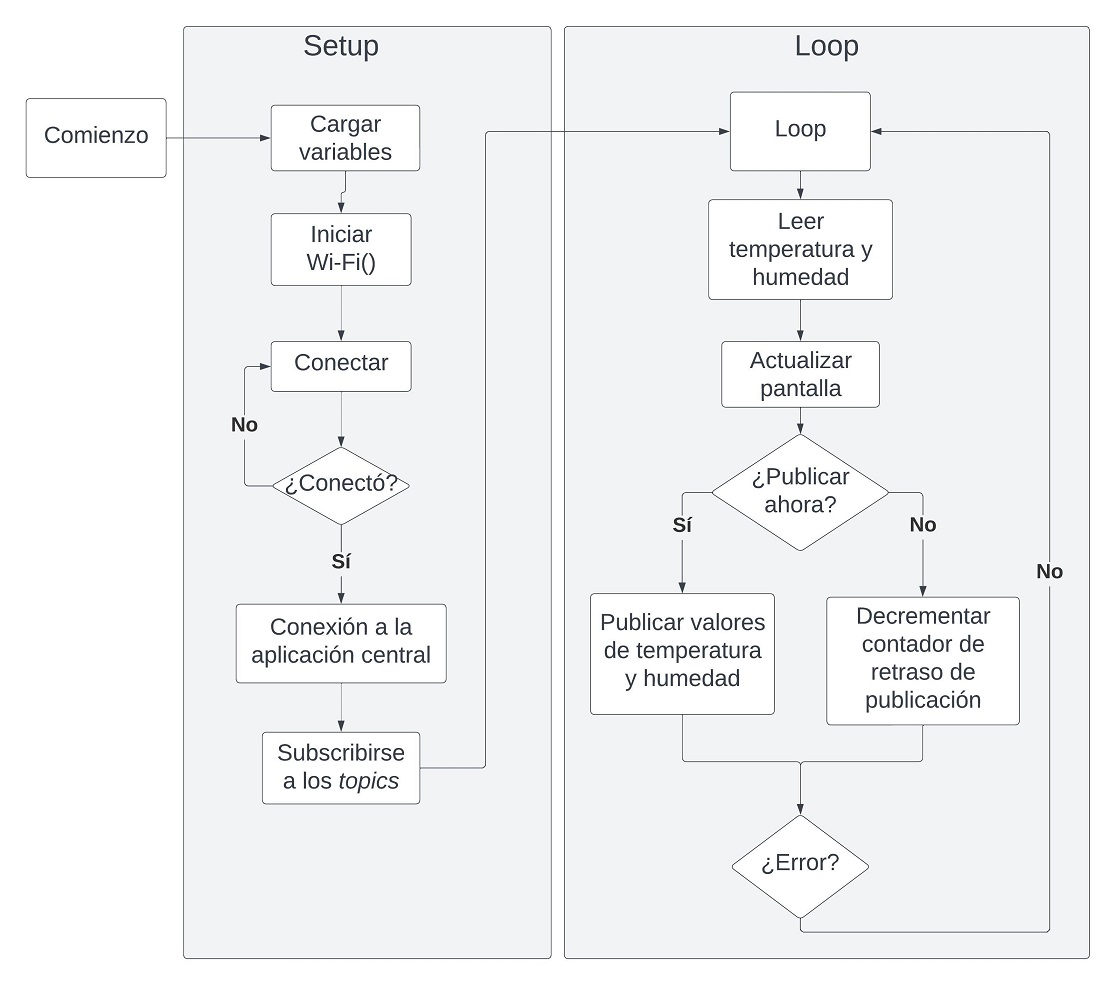
\includegraphics[width=0.8\textwidth]{./Figures/chapter3/FirmwareTempSensor.jpg}
	\caption[Diagrama de flujo del firmware del módulos sensores de temperatura y humedad]{Diagrama de flujo del firmware del módulos sensores de temperatura y humedad.}
	\label{fig:flow_tempsensor}
\end{figure}

\pagebreak
\subsection{Firmware del módulo de control de clima}
\label{Firmware del módulo de control de clima}

Es el que se encarga del encendido y apagado de los ventiladores para el control de clima.
Luego de la comienzo, el programa se conecta a la red, se subscribe en los \textit{topics} correspondientes, y queda a la espera de los mensajes. En el caso de recibir un pedido de reporte, responde con el estado del pin GPIO asociado con el ventilador. Si recibe un pedido de prendido o apagado, realiza la acción correspondiente y retorna al inicio del bucle.


\begin{figure}[!h]
	\centering
	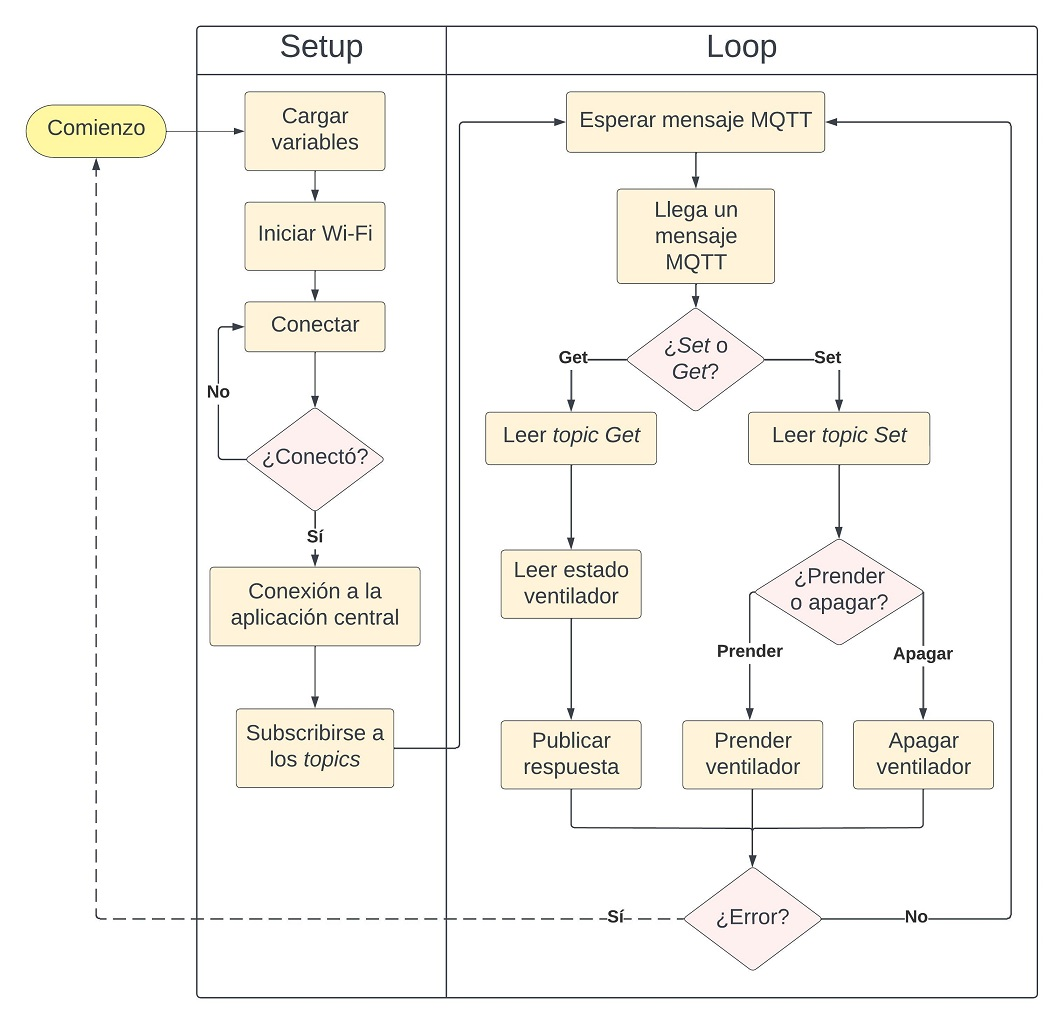
\includegraphics[width=0.8\textwidth]{./Figures/chapter3/FirmwareVentControl.jpg}
	\caption[Diagrama de flujo del firmware del módulo de control de clima]{Diagrama de flujo del firmware del módulo de control de clima.}
	\label{fig:flow_climacontrol}
\end{figure}










\pagebreak
\section{Selección y configuración del software}
\label{sec:Selección y configuración del software}

\textcolor{gray}{A desarrollar: en esta sección explicaré los criterios de selección y configuración del software central como así también el diseño de la interfaz de acceso remoto vía Telegram. }

\section{Ciberseguridad del sistema}
\label{sec:Ciberseguridad del sistema}
\textcolor{gray}{A desarrollar: en esta sección explicaré el uso de TLS en las comunicaciones, las limitaciones encontradas y los riesgos residuales. }


% Chapter Template

\chapter{Ensayos y resultados} % Main chapter title

\label{Chapter4} % Change X to a consecutive number; for referencing this chapter elsewhere, use \ref{ChapterX}

%----------------------------------------------------------------------------------------
%	SECTION 1
%----------------------------------------------------------------------------------------
En este capítulo se explica la metodología de pruebas aplicada tanto a los componentes individuales como al sistema implementado para finalizar con una comparación con el estado del arte.


\section{Banco de pruebas}
\label{sec:Banco de pruebas}
%
%La verificación del correcto funcionamiento de los módulos que componen el sistema se realizó mediante una maqueta que represente en escala reducida al invernadero del cliente.
%El modelo cuenta con una bomba de agua conectada a tres válvulas para simular hasta tres circuitos de riego.
%Para el armado se utilizaron mangueras y conexiones neumáticas de aluminio de acople rápido como muestra la figura \ref{fig:pump}   
%El proceso de construcción de la maqueta se muestra en la figura \ref{fig:invernadero}, allí se observa la implementación de dos circuitos de riego independientes para diferentes clases de macetas y se configuró un tercer circuito cerrado de agua para pruebas de accionamiento de bomba y válvula para evitar desperdicios durante las fases de calibración.
%
%
%\begin{figure}[h]
%	\centering
%	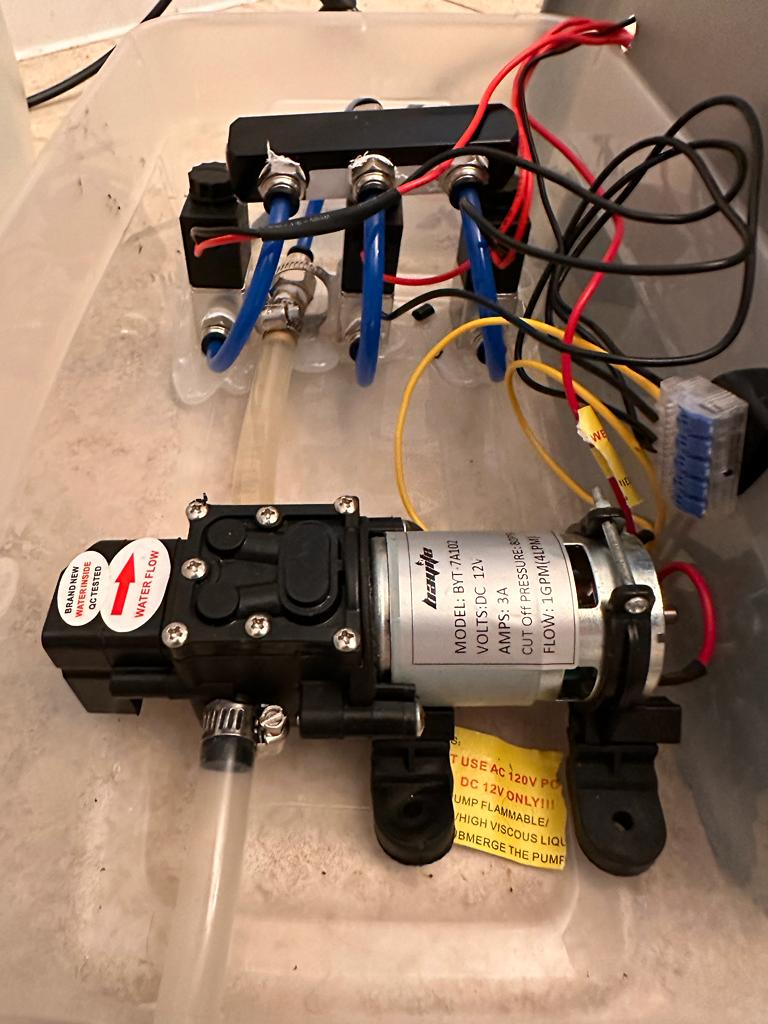
\includegraphics[width=0.5\textwidth]{./Figures/chapter4/pump_2.jpg}
%	\caption[Conexión de bomba y válvulas]{Conexión de bomba y válvulas.}
%	\label{fig:pump}
%\end{figure}
%
%\begin{figure}[!htpb]
%     \centering
%     \begin{subfigure}[b]{0.45\textwidth}
%		\centering
%		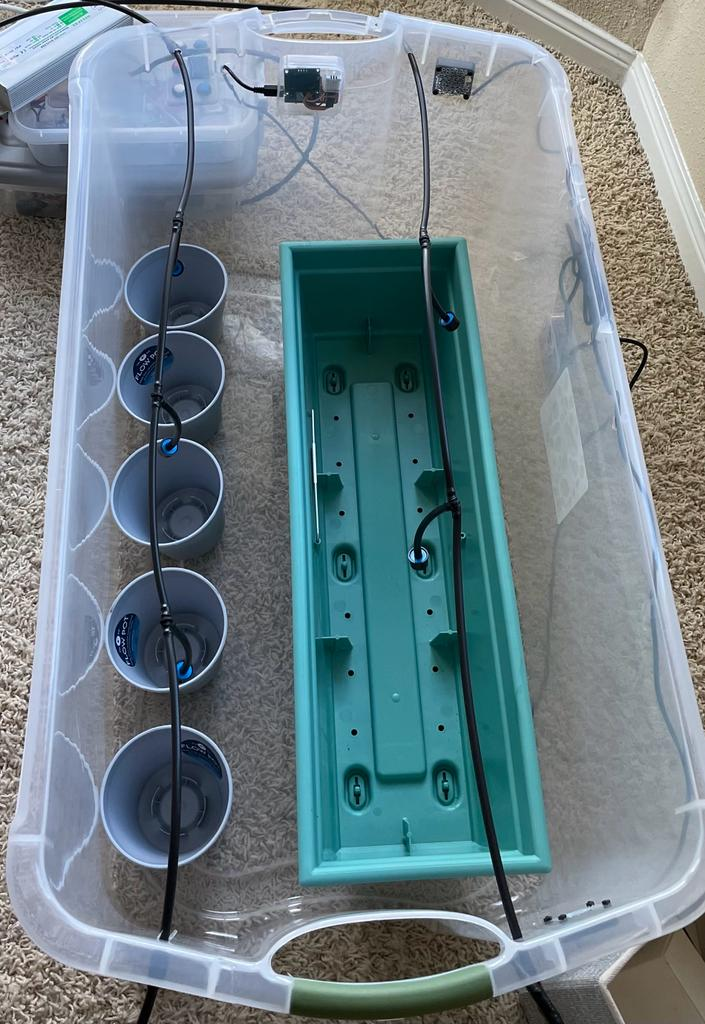
\includegraphics[width=0.70\textwidth]{./Figures/chapter4/Invernadero1.jpg}
%		\caption{Armado de mangueras de riego.}
%		\label{fig:gh1}
%     \end{subfigure}
%     \hfill
%     \begin{subfigure}[b]{0.45\textwidth}
%	    \centering
%		 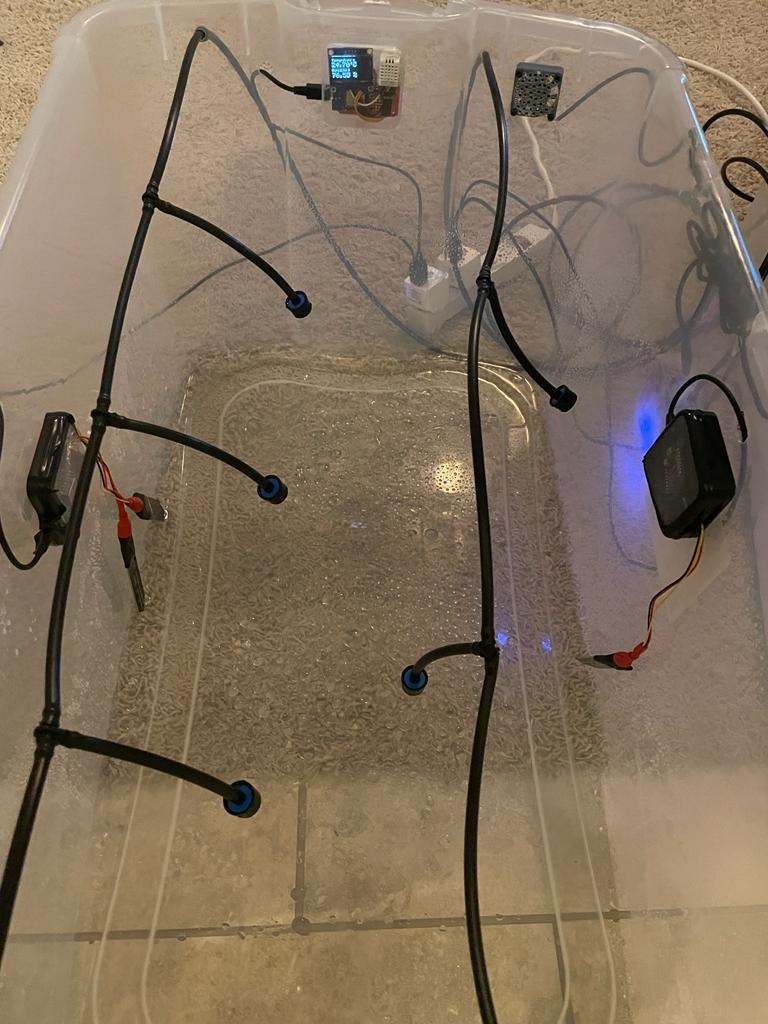
\includegraphics[width=0.75\textwidth]{./Figures/chapter4/Invernadero2.jpg}
%		\caption{Pruebas de riego.}
%		\label{fig:gh2}
%     \end{subfigure}
%     \hfill	
%	 \begin{subfigure}[b]{0.45\textwidth}
%		\centering
%		\includegraphics[width=0.60\textwidth]{./Figures/chapter4/Invernadero3.jpg}
%		\caption{Ensamble general.}
%		\label{fig:gh3}
%     \end{subfigure}
%     \hfill
%%          \begin{subfigure}[b]{0.45\textwidth}
%%		\centering
%%		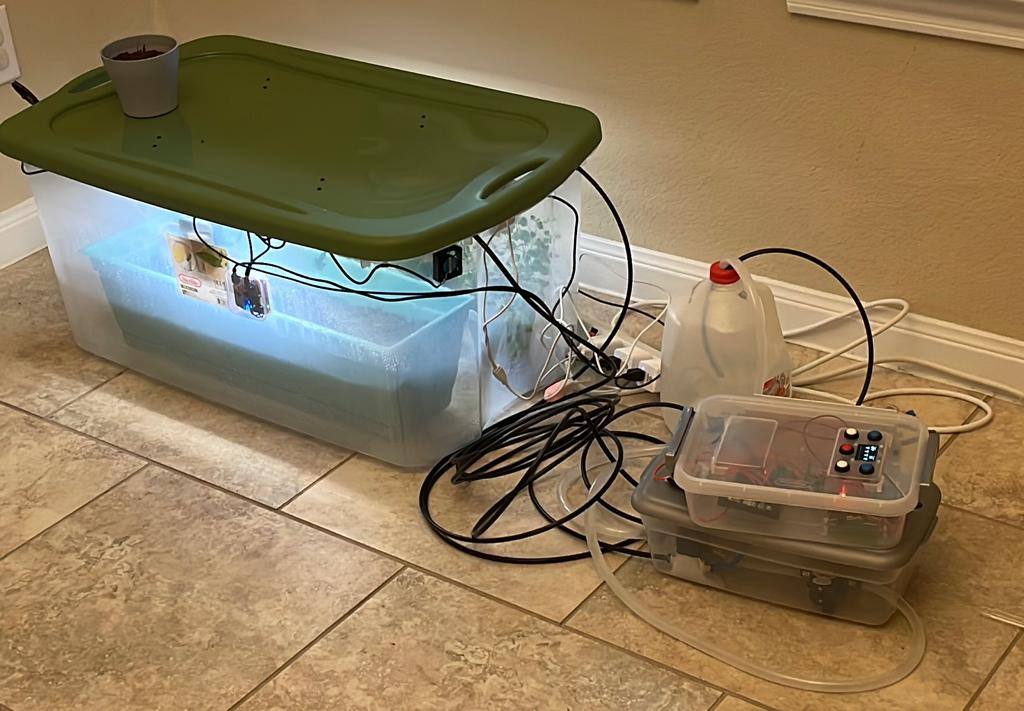
\includegraphics[width=0.90\textwidth]{./Figures/chapter4/Invernadero4.jpg}
%%		\caption{Modelo terminado.}
%%		\label{fig:gh4}
%%     \end{subfigure}
%%     \hfill
%     \begin{subfigure}[b]{0.45\textwidth}
%	    \centering
%		 \includegraphics[width=0.80\textwidth]{./Figures/chapter4/Invernadero5.jpg}
%		\caption{Modelo terminado.}
%		\label{fig:gh5}
%     \end{subfigure}
%     \hfill	
%
%        \caption[Modelo de pruebas del invernadero]{Modelo de pruebas del invernadero.}
%        \label{fig:invernadero}
%\end{figure}
%
%La tabla \ref{tab:herramientas} detalla las diferentes herramientas empleados para la configuración y validación de requerimientos sobre el sistema:
%
%
%
%\begin{table}[h]
%\centering
%\caption[Herramientas empleadas para las pruebas]{Herramientas empleadas para las pruebas.}
%
%%\begin{tabular}{ll} } 
%\begin{tabularx}{\textwidth}{sb}  
%\toprule
%\textbf{Recurso} & \textbf{Función}\\
%
%\midrule
%				&	\tabitem Instalación y configuración de Thingsboard. \\
%Computadora      &   \tabitem Desarrollo y carga del firmware en módulos. \\
%                &   \tabitem Pruebas de acceso y concurrencia al sistema. \\
%Teléfono celular	& Pruebas de acceso y concurrencia al sistema.\\
%Pistola de calor	& Pruebas de control de temperatura. \\
%Recipientes y tierra fértil	&	Calibración de sensores de humedad del suelo.\\ 
%Protoboard y leds	& Pruebas sobre módulos actuadores.\\
%\bottomrule
%\hline
%\end{tabularx}
%\label{tab:herramientas}
%\end{table}

\section{Pruebas unitarias}
\label{sec:Pruebas unitarias}


\section{Pruebas de sistema}
\label{sec:Pruebas de sistema}



\section{Comparativa con el estado de arte}
\label{sec:Comparativa con el estado de arte} 
% Chapter Template

\chapter{Conclusiones} % Main chapter title

\label{Chapter5} % Change X to a consecutive number; for referencing this chapter elsewhere, use \ref{ChapterX}


%----------------------------------------------------------------------------------------

%----------------------------------------------------------------------------------------
%	SECTION 1
%----------------------------------------------------------------------------------------


En este capítulo se muestran las conclusiones sobre el trabajo realizado. A su vez
se presentan algunas modificaciones o mejoras como posible trabajo futuro.
\section{Resultados obtenidos }


En este trabajo se completó el diseño, desarrollo, evaluación e implementación de un
prototipo de sistema escalable que automatiza el control y monitoreo de un invernadero inteligente de tipo hogareño, de acuerdo con el cronograma y los costos establecidos, al tiempo que se lograron satisfacer todos los requerimientos del cliente.

Para su realización fueron de gran utilidad los conocimientos adquiridos a lo largo de la especialización, en particular resaltan:
\begin{itemize}
\item Gestión de proyectos: organizó y facilitó la ejecución de las tareas.
\item Protocolos de IoT: proveyó las bases para el entendimiento de la comunicación entre la capa física y la de aplicación.
\item Ciberseguridad en IoT: brindó herramientas y técnicas para la protección del sistema.
\item Desarrollo de aplicaciones para Internet de las cosas: dio los fundamentos para la programación del firmware y de los protocolos de comunicaciones. 
\end{itemize}



Durante la implementación del prototipo surgieron imprevistos que, si bien fueron resueltos, merecen ser mencionados:
\begin{itemize}
\item El desarrollo en escala introdujo complicaciones en los sistemas hidráulicos, por lo que se debieron emplear mangueras y conectores de alta presión para eliminar los riesgos de roturas.

\item La calibración de los sensores capacitivos de humedad del suelo empleados se basa en una relación lineal entre la capacitancia medida por el sensor y la humedad del suelo \citep{soilcalibration}. Sin embargo, esta ecuación no toma en cuenta otros factores que pueden afectar la medición, tales como la temperatura, la salinidad y la compactación del suelo. Por lo tanto, la precisión del ajuste puede verse comprometida si estos varían en el entorno en el que se encuentra el sensor.

Además, este modelo se basa en una configuración fija del dispositivo y no es fácilmente adaptable. Esto significa que si se desea introducir alguna modificación, resultará necesaria una nueva calibración, lo que puede ser costoso y requerir tiempo adicional.

\item El correcto ajuste de los parámetros del invernadero requiere conocimientos botánicos para asegurar condiciones de riego y temperatura adecuadas para las plantas en cultivo. 
\end{itemize}


\section{Corolario}
Las ofertas disponibles en el mercado generalmente cuentan con una amplia gama de características integradas que pueden hacerlas más atractivas para quienes buscan una solución rápida y lista para usar. Sin embargo, suelen presentar un costo elevado y el usuario queda supeditado a lo que ofrezca el producto y a las posibles ampliaciones determinadas por el fabricante.

%Por el contrario, un invernadero inteligente como el realizado aporta flexibilidad, posibilidades de expansión y adaptabilidad a dispositivos que se desarrollen o adopten a futuro. Bastará con elegir y configurar los nuevos módulos sensores y dispositivos a utilizar en el sistema, lo que puede requerir un mayor esfuerzo y conocimientos técnicos.

En cambio, un invernadero inteligente como el que se ha construido proporciona flexibilidad, opciones de crecimiento y capacidad de adaptación a futuros componentes que se desarrollen o adopten. Para lograrlo, simplemente se necesitará seleccionar y configurar los nuevos sensores y herramientas a utilizar en el sistema, lo que puede requerir un mayor esfuerzo y conocimientos técnicos.






%----------------------------------------------------------------------------------------
%	SECTION 2
%----------------------------------------------------------------------------------------
\section{Trabajo futuro}

Para dar continuidad al esfuerzo realizado hasta el momento y poder obtener un producto más completo, se proponen las siguientes mejoras:

\begin{itemize}
\item Evaluar el rediseño o compra de los módulos físicos a fin de unificar los componentes electrónicos internos en una placa de circuito impreso más pequeña. %, considerando estándares de fabricación de placas electrónicas para uso comercial.
 
\item Configurar una red de tipo \textit{ad hoc} sobre la placa inalámbrica de la Raspberry Pi y emplear la red Ethernet para el acceso a Internet, de forma de separar las redes personales de la del invernadero.

\item Evaluar diferentes opciones que permitan garantizar autenticación basada en certificados entre los dispositivos y la aplicación, como así también entre los usuarios y la aplicación, para reducir exposiciones.

\item Continuar el análisis sobre la medición de humedad del suelo mediante sensores capacitivos, para identificar mejoras o simplificaciones en la calibración, conforme se varíe el tipo de suelo y plantas a cultivar. 

\item Expandir el sistema para agregar nuevos actuadores, tales como tomacorrientes que sean controlados por la aplicación. Mediante los cuales puedan incorporarse nuevos subsistemas, entre los que se encuentran humidificadores y luces. 

\end{itemize} 

%----------------------------------------------------------------------------------------
%	CONTENIDO DE LA MEMORIA  - APÉNDICES
%----------------------------------------------------------------------------------------

\appendix % indicativo para indicarle a LaTeX los siguientes "capítulos" son apéndices

% Incluir los apéndices de la memoria como archivos separadas desde la carpeta Appendices
% Descomentar las líneas a medida que se escriben los apéndices

%% Appendix A

\chapter{Appendix Title Here} % Main appendix title

\label{AppendixA} % For referencing this appendix elsewhere, use \ref{AppendixA}

Write your Appendix content here.
%\include{Appendices/AppendixB}
%\include{Appendices/AppendixC}

%----------------------------------------------------------------------------------------
%	BIBLIOGRAPHY
%----------------------------------------------------------------------------------------

\Urlmuskip=0mu plus 1mu\relax
\raggedright
\printbibliography[heading=bibintoc]

%----------------------------------------------------------------------------------------

\end{document}  
